\documentclass[11pt,a4paper,]{article}
\usepackage{lmodern}

\usepackage{amssymb,amsmath}
\usepackage{ifxetex,ifluatex}
\usepackage{fixltx2e} % provides \textsubscript
\ifnum 0\ifxetex 1\fi\ifluatex 1\fi=0 % if pdftex
  \usepackage[T1]{fontenc}
  \usepackage[utf8]{inputenc}
\else % if luatex or xelatex
  \usepackage{unicode-math}
  \defaultfontfeatures{Ligatures=TeX,Scale=MatchLowercase}
\fi
% use upquote if available, for straight quotes in verbatim environments
\IfFileExists{upquote.sty}{\usepackage{upquote}}{}
% use microtype if available
\IfFileExists{microtype.sty}{%
\usepackage[]{microtype}
\UseMicrotypeSet[protrusion]{basicmath} % disable protrusion for tt fonts
}{}
\PassOptionsToPackage{hyphens}{url} % url is loaded by hyperref
\usepackage[unicode=true]{hyperref}
\hypersetup{
            pdftitle={Predicting Critical Elements in Coal Mine Waste: A Machine Learning Approach for a Low-Emission Future},
            pdfborder={0 0 0},
            breaklinks=true}
\urlstyle{same}  % don't use monospace font for urls
\usepackage{geometry}
\geometry{a4paper, centering, text={16cm,25cm}}
\usepackage[style=authoryear-comp,]{biblatex}
\addbibresource{references.bib}
\usepackage{longtable,booktabs}
% Fix footnotes in tables (requires footnote package)
\IfFileExists{footnote.sty}{\usepackage{footnote}\makesavenoteenv{long table}}{}
\usepackage{graphicx,grffile}
\makeatletter
\def\maxwidth{\ifdim\Gin@nat@width>\linewidth\linewidth\else\Gin@nat@width\fi}
\def\maxheight{\ifdim\Gin@nat@height>\textheight\textheight\else\Gin@nat@height\fi}
\makeatother
% Scale images if necessary, so that they will not overflow the page
% margins by default, and it is still possible to overwrite the defaults
% using explicit options in \includegraphics[width, height, ...]{}
\setkeys{Gin}{width=\maxwidth,height=\maxheight,keepaspectratio}
\IfFileExists{parskip.sty}{%
\usepackage{parskip}
}{% else
\setlength{\parindent}{0pt}
\setlength{\parskip}{6pt plus 2pt minus 1pt}
}
\setlength{\emergencystretch}{3em}  % prevent overfull lines
\providecommand{\tightlist}{%
  \setlength{\itemsep}{0pt}\setlength{\parskip}{0pt}}
\setcounter{secnumdepth}{5}

% set default figure placement to htbp
\makeatletter
\def\fps@figure{htbp}
\makeatother


\title{Predicting Critical Elements in Coal Mine Waste: A Machine Learning Approach for a Low-Emission Future}

%% MONASH STUFF

%% CAPTIONS
\RequirePackage{caption}
\DeclareCaptionStyle{italic}[justification=centering]
 {labelfont={bf},textfont={it},labelsep=colon}
\captionsetup[figure]{style=italic,format=hang,singlelinecheck=true}
\captionsetup[table]{style=italic,format=hang,singlelinecheck=true}


%% FONT
\RequirePackage{bera}
\RequirePackage[charter,expert,sfscaled]{mathdesign}
\RequirePackage{fontawesome}

%% HEADERS AND FOOTERS
\RequirePackage{fancyhdr}
\pagestyle{fancy}
\rfoot{\Large\sffamily\raisebox{-0.1cm}{\textbf{\thepage}}}
\makeatletter
\lhead{\textsf{\expandafter{\@title}}}
\makeatother
\rhead{}
\cfoot{}
\setlength{\headheight}{15pt}
\renewcommand{\headrulewidth}{0.4pt}
\renewcommand{\footrulewidth}{0.4pt}
\fancypagestyle{plain}{%
\fancyhf{} % clear all header and footer fields
\fancyfoot[C]{\sffamily\thepage} % except the center
\renewcommand{\headrulewidth}{0pt}
\renewcommand{\footrulewidth}{0pt}}

%% MATHS
\RequirePackage{bm,amsmath}
\allowdisplaybreaks

%% GRAPHICS
\RequirePackage{graphicx}
\setcounter{topnumber}{2}
\setcounter{bottomnumber}{2}
\setcounter{totalnumber}{4}
\renewcommand{\topfraction}{0.85}
\renewcommand{\bottomfraction}{0.85}
\renewcommand{\textfraction}{0.15}
\renewcommand{\floatpagefraction}{0.8}


%\RequirePackage[section]{placeins}

%% SECTION TITLES


%% SECTION TITLES
\RequirePackage[compact,sf,bf]{titlesec}
\titleformat*{\section}{\Large\sf\bfseries\color[rgb]{0.7,0,0}}
\titleformat*{\subsection}{\large\sf\bfseries\color[rgb]{0.7,0,0}}
\titleformat*{\subsubsection}{\sf\bfseries\color[rgb]{0.7,0,0}}
\titlespacing{\section}{0pt}{2ex}{.5ex}
\titlespacing{\subsection}{0pt}{1.5ex}{0ex}
\titlespacing{\subsubsection}{0pt}{.5ex}{0ex}


%% TITLE PAGE
\def\Date{\number\day}
\def\Month{\ifcase\month\or
 January\or February\or March\or April\or May\or June\or
 July\or August\or September\or October\or November\or December\fi}
\def\Year{\number\year}

%% LINE AND PAGE BREAKING
\sloppy
\clubpenalty = 10000
\widowpenalty = 10000
\brokenpenalty = 10000
\RequirePackage{microtype}

%% PARAGRAPH BREAKS
\setlength{\parskip}{1.4ex}
\setlength{\parindent}{0em}

%% HYPERLINKS
\RequirePackage{xcolor} % Needed for links
\definecolor{darkblue}{rgb}{0,0,.6}
\RequirePackage{url}

\makeatletter
\@ifpackageloaded{hyperref}{}{\RequirePackage{hyperref}}
\makeatother
\hypersetup{
     citecolor=0 0 0,
     breaklinks=true,
     bookmarksopen=true,
     bookmarksnumbered=true,
     linkcolor=darkblue,
     urlcolor=blue,
     citecolor=darkblue,
     colorlinks=true}

\usepackage[showonlyrefs]{mathtools}
\usepackage[no-weekday]{eukdate}

%% BIBLIOGRAPHY

\makeatletter
\@ifpackageloaded{biblatex}{}{\usepackage[style=authoryear-comp, backend=biber, natbib=true]{biblatex}}
\makeatother
\ExecuteBibliographyOptions{bibencoding=utf8,minnames=1,maxnames=3, maxbibnames=99,dashed=false,terseinits=true,giveninits=true,uniquename=false,uniquelist=false,doi=false, isbn=false,url=true,sortcites=false}

\DeclareFieldFormat{url}{\texttt{\url{#1}}}
\DeclareFieldFormat[article]{pages}{#1}
\DeclareFieldFormat[inproceedings]{pages}{\lowercase{pp.}#1}
\DeclareFieldFormat[incollection]{pages}{\lowercase{pp.}#1}
\DeclareFieldFormat[article]{volume}{\mkbibbold{#1}}
\DeclareFieldFormat[article]{number}{\mkbibparens{#1}}
\DeclareFieldFormat[article]{title}{\MakeCapital{#1}}
\DeclareFieldFormat[article]{url}{}
%\DeclareFieldFormat[book]{url}{}
%\DeclareFieldFormat[inbook]{url}{}
%\DeclareFieldFormat[incollection]{url}{}
%\DeclareFieldFormat[inproceedings]{url}{}
\DeclareFieldFormat[inproceedings]{title}{#1}
\DeclareFieldFormat{shorthandwidth}{#1}
%\DeclareFieldFormat{extrayear}{}
% No dot before number of articles
\usepackage{xpatch}
\xpatchbibmacro{volume+number+eid}{\setunit*{\adddot}}{}{}{}
% Remove In: for an article.
\renewbibmacro{in:}{%
  \ifentrytype{article}{}{%
  \printtext{\bibstring{in}\intitlepunct}}}

\AtEveryBibitem{\clearfield{month}}
\AtEveryCitekey{\clearfield{month}}

\makeatletter
\DeclareDelimFormat[cbx@textcite]{nameyeardelim}{\addspace}
\makeatother

\author{\sf{\Large\textbf{Evan Ginting}\\\large Master of Business Analytics\newline 33477558 \newline \href{mailto:egin0003@student.monash.edu}{\nolinkurl{egin0003@student.monash.edu}}\\[0.5cm]}{\Large\textbf{Yuhao Long}\\\large Master of Business Analytics\newline 33412448 \newline \href{mailto:ylon0012@student.monash.edu}{\nolinkurl{ylon0012@student.monash.edu}}\\[0.5cm]}{\Large\textbf{Dr Kane Maxwell}\\\large Matrix Geoscience \newline \href{mailto:kane.maxwell@matrixgeoscience.com}{\nolinkurl{kane.maxwell@matrixgeoscience.com}}\\[0.5cm]}{\Large\textbf{Limin Xu}\\\large Matrix Geoscience \newline \href{mailto:limin.xu@matrixgeoscience.com}{\nolinkurl{limin.xu@matrixgeoscience.com}}\\[0.5cm]}}

\date{\sf\Date~\Month~\Year}
\makeatletter
\lfoot{\sf Ginting, Long, Maxwell, Xu: \@date}
\makeatother


%%%% PAGE STYLE FOR FRONT PAGE OF REPORTS

\makeatletter
\def\organization#1{\gdef\@organization{#1}}
\def\telephone#1{\gdef\@telephone{#1}}
\def\email#1{\gdef\@email{#1}}
\makeatother
  \organization{ETC5543}

  \def\name{Department of\newline Econometrics \&\newline Business Statistics}

  \telephone{(03) 9905 2478}

  \email{\href{mailto:BusEco-Econometrics@monash.edu}{\nolinkurl{BusEco-Econometrics@monash.edu}}}

\def\webaddress{\url{http://buseco.monash.edu/ebs/consulting/}}
\def\abn{12 377 614 012}
\def\extraspace{\vspace*{1.6cm}}
\makeatletter
\def\contactdetails{\faicon{phone} & \@telephone \\
                    \faicon{envelope} & \@email}
\makeatother

\usepackage[absolute,overlay]{textpos}
\setlength{\TPHorizModule}{1cm}
\setlength{\TPVertModule}{1cm}

%%%% FRONT PAGE OF REPORTS

\def\reporttype{Report for}

\long\def\front#1#2#3{
\newpage
\begin{textblock}{7}(12.7,28.2)\hfill

\includegraphics[height=0.6cm]{AACSB}~~~

\includegraphics[height=0.6cm]{EQUIS}~~~

\includegraphics[height=0.6cm]{AMBA}
\end{textblock}
\begin{singlespacing}
\thispagestyle{empty}
\vspace*{-1.4cm}
\hspace*{-1.4cm}
\hbox to 16cm{
  \hbox to 6.5cm{\vbox to 14cm{\vbox to 25cm{
    
\includegraphics[width=6cm]{monash2}
    \vfill
    
\includegraphics[width=3.5cm]{MBSportrait}
    \vspace{0.4cm}
    \par
    \parbox{6.3cm}{\raggedright
      \sf\color[rgb]{0.00,0.00,0.70}
      {\large\textbf{\name}}\par
      \vspace{.7cm}
      \tabcolsep=0.12cm\sf\small
      \begin{tabular}{@{}ll@{}}\contactdetails
      \end{tabular}
      \vspace*{0.3cm}\par
      ABN: \abn\par
    }
  }\vss}\hss}
  \hspace*{0.2cm}
  \hbox to 1cm{\vbox to 14cm{\rule{1pt}{26.8cm}\vss}\hss\hfill}
  \hbox to 10cm{\vbox to 14cm{\vbox to 25cm{
      \vspace*{3cm}\sf\raggedright
      \parbox{11cm}{\sf\raggedright\baselineskip=1.2cm
         \fontsize{24.88}{30}\color[rgb]{0.70,0.00,0.00}\sf\textbf{#1}}
      \par
      \vfill
      \large
      \vbox{\parskip=0.8cm #2}\par
      \vspace*{2cm}\par
      \reporttype\\[0.3cm]
      \hbox{#3}%\\[2cm]\
      \vspace*{1cm}
      {\large\sf\textbf{\Date~\Month~\Year}}
   }\vss}
  }}
\end{singlespacing}
\newpage
}

\makeatletter
\def\titlepage{\front{\expandafter{\@title}}{\@author}{\@organization}}
\makeatother

\usepackage{setspace}
\setstretch{1.5}

%% Any special functions or other packages can be loaded here.
\usepackage{float} \floatplacement{figure}{H} \usepackage{colortbl} \usepackage{color}
\usepackage{booktabs}
\usepackage{longtable}
\usepackage{array}
\usepackage{multirow}
\usepackage{wrapfig}
\usepackage{float}
\usepackage{colortbl}
\usepackage{pdflscape}
\usepackage{tabu}
\usepackage{threeparttable}
\usepackage{threeparttablex}
\usepackage[normalem]{ulem}
\usepackage{makecell}
\usepackage{xcolor}


\begin{document}
\titlepage

{
\setcounter{tocdepth}{1}
\tableofcontents
}
\newpage

\section{Abstract}\label{abstract}

As global demand for critical minerals rises, this study investigates the economic potential of extracting critical elements from coal mine waste in Australia. Using data from the largest element mapping project by ACARP, combined with recent private sector research, this research employs Exploratory Data Analysis (EDA) and machine learning to achieve two key objectives: (1) leveraging low-cost lab analysis (ME-4ACD81) to predict concentrations of valuable elements such as REEs (Rare Earth Element), HREEs (Heavy Rare Earth Element), and LREEs (Light Rare Earth Element) through numerical regression, and (2) identifying enriched elements and project areas with significant economic potential for future extraction. The study found that elements from low-cost lab analysis can predict the REEs, HREEs, and LREEs with reasonably good performance. This was achieved even with the challenge of low correlation coefficient between the independent and dependent variables. This study also found that Fort Cooper possess a significant amount of critical elements, making it economically feasible to pursue extraction efforts with confidence that the investment in Fort Cooper will yield substantial returns and contribute meaningfully to meeting the global demand for critical minerals.

\section{Background and Motivation}\label{background-and-motivation}

\subsection{Critical elements overview}\label{critical-elements-overview}

In this technology advancement era where mineral-based technologies are relied by many industrial sectors, critical elements become highly-sought elements in the world \autocite{Emsbo2021}. Critical elements can be defined by two main criteria: first, elements that are essential for manufacturing modern technologies, supporting economic frameworks, and ensuring national security; and second, elements with vulnerable supply chains, which can be affected by political issues, geographic concentration of extraction or production, and natural disasters \autocite{Lian2024,Fortier2018,DISR2023}.

According to \href{https://www.industry.gov.au/publications/critical-minerals-strategy-2023-2030}{Critical Minerals Strategy 2023--2030} \autocite{geoscience2023}, fifteen elements have been identified as highly vulnerable to future supply chain disruptions and additional fifteen elements as moderate risk, which defined in \hyperref[sec-appendixone]{Appendix 1} \autocite{Coyne2023,Skirrow2013,IEA2024b,Fortier2018,Austrade2024}. Among these critical elements, Rare Earth Elements (REE) represent a significant subset. REEs are a group of seventeen chemically similar metallic elements composed of fifteen lanthanides, scandium, and yttrium. They further grouped into heavy (HREEs) and light (LREEs) based on their atomic number, electron arrangement, and chemical properties \autocite{Reid2018}.

Global initiatives to reduce carbon emissions by transitioning to clean energy have led to increasing demand for critical elements, which are essential resources for achieving this goal \autocite{IEA2021,Wang2022}. According to \textcite{IEA2024} research, demand for these elements is projected to double, triple, or even quadruple, depending on the scenario, relative to current production levels. Among these elements, lithium is experiencing the most rapid growth due to rising demand for electric vehicle (EV) batteries, while copper leads in terms of production volume. Graphite demand is expected to almost quadruple, and the demand for nickel, cobalt, and REEs is projected to double. Furthermore, \textcite{Fortier2018} indicates that the growing reliance on critical elements is also driven by their applications across various key sectors, including energy, defense, communications, healthcare, transportation, and agriculture. These dynamics have intensified competition to discover new sources and establish stable, long-term supply chains for these vital resources \autocite{Emsbo2021}. The prominent usage of each element and its projected demand are also detailed in \hyperref[sec-appendixone]{Appendix 1}.

As one of the promising top global producers of these critical elements, Australia, with its abundant deposit and technological expertise, plays a pivotal role in the sustainable energy transition and supply chain stability. Australia is the largest producer of lithium, the third largest producer of cobalt, and the fourth largest producer of REEs. It also produces significant amounts of aluminium, nickel, and copper, which are essential for low-emission technologies like electric vehicles, solar panels, and wind turbines \autocite{DISR2023}. Australia's Government strategy to ensure the fulfillment of this potential has been proactive and multifaceted, especially in the past 5 years. The strategy include a range of incentives, finance facilities, grants and other support for the critical elements sector. Some of the important initiatives as reported in \textcite{DISR2023}, are:

1). The Australian Government's Critical Minerals Facility, with AUD 4 billion budget, supports projects that are aligned with the nation's Critical Minerals Strategy and serve the national interest.

2). The Northern Australia Infrastructure Facility (NAIF) allocates up to AUD 500 million of the AUD 5 billion to help finance projects in the Northern Territory, Queensland, and Western Australia.

3). The Junior Minerals Exploration Incentive (JMEI) promotes investment in small minerals-exploration firms that focus on greenfield exploration.

4). Australian federal, state and territory government authorities are collaborating on the AUD 10 million Critical Minerals National Productivity Initiative to develop pre-feasibility studies of common-user infrastructure for the critical elements sector.

5). The Major Projects Facilitation Agency (MPFA) supports developers of projects over AUD 20 million by providing information on Australian Government regulations and approvals, mapping out critical approval processes, and communicating with regulators to address issues.

6). The Critical Minerals Production Tax Incentive offers a production incentive worth ten percent of relevant processing and refining costs for Australia's critical elements. This incentive is available for up to ten years per project for production between 2027--28 and 2039--40, provided the projects reach final investment decisions by 2030.

\subsection{Critical elements in coals}\label{critical-elements-in-coals}

The green technology initiatives and commitments by countries worldwide for decarbonisation have led to a growing market of clean energy and technology. As a result, critical elements, including REEs, are projected to be in high demand in the future \autocite{usde2017}. Currently, China leads the world in REE production, dominating the international trade and global value chain of rare earths \autocite{us2024mineral}. However, their recent export restrictions on REE have led to a disruption in the global supply chain \autocite{MANCHERI2015262}. In response, there is an increasing focus on identifying alternative sources of critical elements, with coal being explored as a potential new source of critical elements \autocite{Hodgkinson2021}.

\hyperref[sec-appendixtwo]{Appendix 2} provides element mapping of the Bowen Basin, the largest coal reserve in Australia, based on \textcite{Hodgkinson2020} study. The concentration of element composition is more influenced by the lithology of the samples than by depth gradation:

1). In coal and its derivatives, although the majority of element concentrations fall below the benchmark when compared to Post-Archaean Australian Shales (PAAS) standard \autocite{McLennan2011}, a widely used geochemical reference material in the average shale compositions, local samples show enrichment in REEs. Additionally, concentrations of bismuth (Bi) are abnormally elevated, showing levels 4-6 times higher than the crustal average.

2). Siltstone and mudstone yield unremarkable results in terms of elemental enrichment, with most element concentrations failing to meet significant thresholds. However, the concentration of cobalt (Co) compounds approaches the crustal average, suggesting potential economic value that warrants further investigation.

3). Tuffaceous rock, formed from volcanic ash, is rich in pumice and lithic fragments. Samples reveal elevated concentrations of strategic elements, including REEs, gallium (Ga), and bismuth (Bi). Moreover, a potentially lithium-rich borehole has been identified, with lithium concentrations approximately five times higher than the crustal average.

\subsection{Economic concentrations}\label{economic-concentrations}

Before the recent surge in demand, extracting critical elements from coal was considered costly, however, methods have been developed that reduce the cost and also enviromentally friendly. Coal and coal byproducts are substantially enhanced with trace metals and have been proposed as a potential source \autocite{Eterigho2021}. A report by US Department of Energy suggests that extracting critical elements from coal material already mined for other purposes, either as a dual product or byproduct, could be more cost-effective than a dedicated mine. Despite the challenge of processing large volumes to obtain economic concentrations, cost may be reduced due to the pre-processed (mined, crushed, and washed) state of the materials and transported to areas with existing infrastructure \autocite{usde2017,Hodgkinson2021}. Based on research, the elements and metals in coal that are considered to have the best chance for economic recovery are: REEs, Ag, Au, PGEs, Be, Se, V, Ga, Sb, Sc, Mo, W, Re, Ge, U, Y, Nb, Zr, Al \autocite{DAI2018155}.

Efficient extraction of critical elements from coal or coal ash, and finding coal sources with highly elevated concentrations of these elements, are essential prerequisites. The value of the element in any coal sources largely determined by their concentration, which varies based on geological and geochemical conditions. Therefore, to economically recovering critical elements from coal is by identifying sources with the highest critical elements levels and accessibility before proceeding to extraction and recovery stages \autocite{Eterigho2021}. \textcite{Reid2018} in his report suggests that critical elements average level in coal is typically just 35 ppm, which is insufficient for economic extraction. While \textcite{Seredin2012} in their reports suggests that a cutoff grade for Rare Earth Oxides (ROE) for coal seam has been suggested as 800-900 ppm. \hyperref[sec-appendixthree]{Appendix 3} provide suggested cut-off grade for 18 critical elements. Additionally, \textcite{TALAN2022107897} reports that coal sources are often relatively enriched in the heavy rare earths (HREEs, Ho, Er, Tm, Yb, Lu) and critical rare earths (CREEs, Y, Nd, Dy, Eu, Tb) compared to traditional mineral deposits. A cut-off grade of 115--130 ppm rare earth element on a whole mass basis may be considered economical. However, the U.S. Department of Energy set a criterion in their work assessing raw coal with total rare earth element content greater than 300 ppm on a whole dry coal basis.

\subsection{Existing economic deposits}\label{existing-economic-deposits}

Currently, there are no coal mines or coal basins extracting critical elements at a commercial states. Most sources found conclude that we are still in the research and development process \autocite{Hodgkinson2020,DAI2018155,Eterigho2021,osti_1808639,TALAN2022107897}. A report by \textcite{Eterigho2021} suggests that the research and development are primarily at the laboratory and pilot scale stages. For example, scholars like Honaker and coworkers who have significant experience in this subject, have constructed a 0.23 t/h solid feed pilot plant for testing different coal-based feedstocks \autocite{osti_1808639}. However, commercial-scale extraction processes have not yet been widely implemented. \textcite{TALAN2022107897} report support this finding as well. They propose a potential approach for commercial-scale extraction of critical elements, indicating ongoing effort to bridge the gap between laboratory research and commercial application. Additionally, they note that further validation and techno-economic analysis are required before these processes can be scaled up commercially. Furthermore, scholars who focusing their research on China's coal resources also suggest further research is needed to scale up the extraction process \autocite{Qin2015,Qin2015b,Liu2024,Zhao2019,ZOU2023105245}. Given that China is the leader in critical elements production, this fact indicates that their production of critical elements does not primarily come from coal and its byproducts.

We can conclude that significant research and development efforts have been made towards commercial extraction of critical elements from coal and coal byproducts. However, it is still long way from actual large-scale implementation. Most scholars indicate the necessity of considering sustainability factors. Effective waste management and treatment, along with the evaluation of extraction costs and technical feasibility, are important. At the end of the day, these elements are going to be utilised in green technology initiatives, such as renewable energy systems and electric vehicles, which demand high-purity materials. Ensuring that their extraction processes are environmentally and economically sustainable is crucial to align with the goals of these green technologies initiatives. Furthermore, ongoing research is vital to bridge existing technology gaps and develop robust, scalable methods that can transition from pilot projects to commercial operations.

\subsection{Extraction of critical elements}\label{extraction-of-critical-elements}

There are several stages required for critical elements to be extracted from coal and coal byproducts. First, Coal and coal byproducts are prepared by crushing and milling to separate the organic from inorganic elements, to generate fine concentrates. These concentrates then undergo further separation techniques, such as physical (froth flotation, electrostatic, magnetic, gravity) and chemical (leaching) methods. Subsequently, they are further processed into purification to extract the REE into pure oxide form (e.g.~REO). While REOs can be standalone products, market demand often dictates their conversion into metals. Thus, in the refining stage, REOs are converted into high-purity rare earth metals using electrolysis or metallothermic reduction processes. These metals may then be alloyed with other elements to enhance their hardness and strength for the end-use market \autocite{Eterigho2021,usde2017,TALAN2022107897}. Figure \ref{fig:ree-vc} visualise this process.

\begin{figure}

{\centering 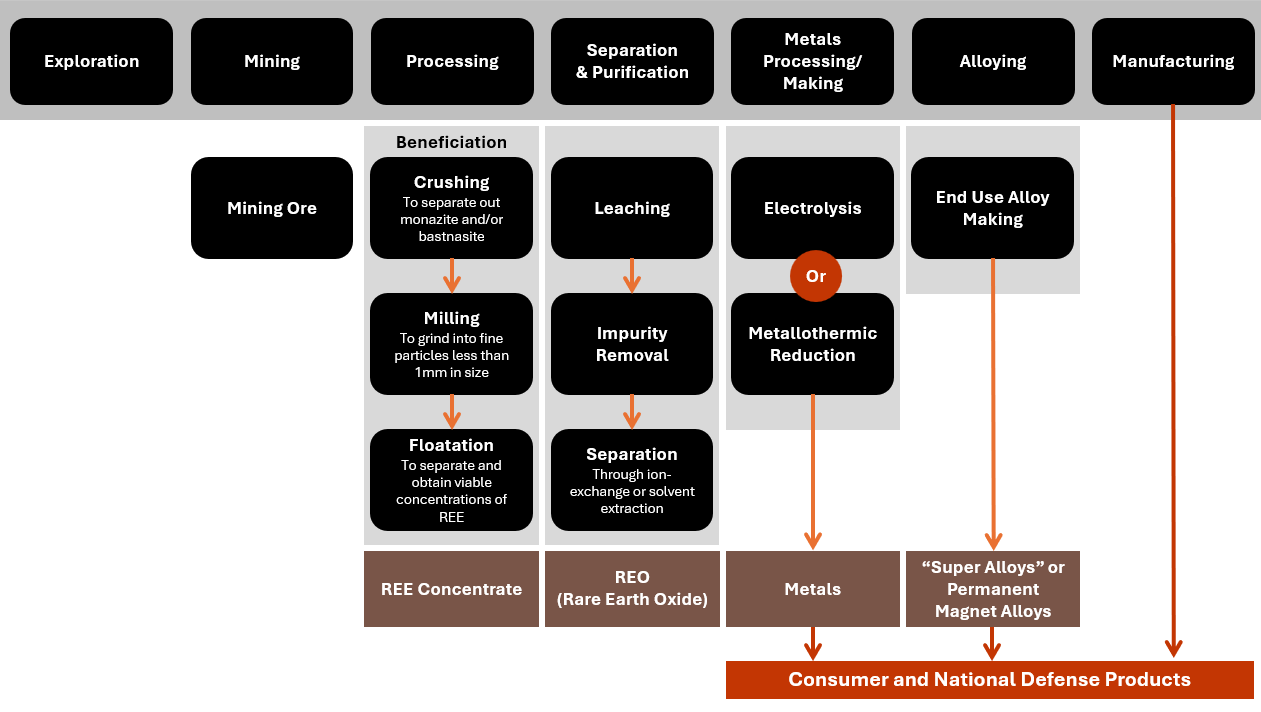
\includegraphics[width=1\linewidth]{Final_report_files/figure-latex/Critical_Mineral_Extraction_Process_v2} 

}

\caption{REE Value Chain (Source: US Department of Energy, 2017)}\label{fig:ree-vc}
\end{figure}

Recently, water-leaching is a prevailing approach since it mitigate the flaw from traditional techniques. Water leaching can be considered as less environmentally detrimental compared to strong acid/alkaline leaching, as well as cost effective for solvent selection. The crucial stages on this preparation workflow are low temperature activation and water leaching. During the stage of low temperature activation, the chemical reaction within coal fly ash (CFA) will be facilitated by complexation agents (ammonium salts or weak acids) in covered alumina crucibles, which help liberate critical elements from the matrix of the CFA. After the activation and cool down to ambient temperature, the tablets are placed in water for the leaching and dissolve process. Water acts as the leaching solvent, extracting these soluble elements into the leachate.The configuration in temperature and mass ratio of solvent will be the vital determinant for optimized recovery. Take Lithium example, it can achieve a stable leaching efficiency of 90\% through ammonium fluoride leaching at 150°C with a \(SiO_2/NH_4F\) mass ratio of 1:1.35 \textcite{Xu2021}.

Another innovation is Hydrophobic-Hydrophilic Separation (HHS), designed to leverages the disparity of affinity (water-repellent \& water-friendly) properties of substances to achieve separation.It can treat as a complementary application for small particle delamination without size limit, providing flexible and extensible purpose in the segregation of ultrafine coal \textcite{Hodgkinson2021}.

In precious \textcite{Hodgkinson2020} element mapping project on Bowen basin,the largest coal reserves in Australia, the concentration of element composition is subjective to sample's lithology rather than the depth grading:

1). In coal and derivative, albeit majority of element concentrations is inferior of the benchmark against earth crust average, local samples exhibit enrichment in HREE and Scandium in respect to \textcite{McLennan2011} Post-Archaean Australian Shales (PAAS) standard , while abnormal 4-6 times higher than crustal average in moderate critical element, Bismuth(Bi) .

2). Siltstone and mudstone has a lackluster finding to classify enrichment for majority of elements concentration,except for the concentration of Cobalt compound barely meet crustal average, whose ubiquitous economic value may warrant further examination.

3). As the sediment from volcanic ash, tuffaceous rock is rich in pumice and lithic fragments. The sample display a series of elevated concentrations of strategic elements including REE, Ga and Bi. Besides, a potential Lithium-rich borehole is found, with approximate 5 times higher than crustal average.

\section{Objectives and Significance}\label{objectives-and-significance}

The primary objective of this study is to develop a predictive model using machine learning to identify and quantify critical minerals---such as copper, lithium, nickel, cobalt, and rare earth elements---in coal mine waste. By analysing existing coal data, this study aims to provide valuable insights into the potential recovery of these essential minerals from coal deposits, contributing to waste reduction and supporting the transition to low-emission technologies. The outcome of this study will help assess the economic value of these minerals and promote sustainable practices within the mining and energy sectors.

The study utilises multiple datasets, some of which are publicly available while others are confidential. The public dataset was released by the Australian Coal Industry's Research Program (ACARP) in 2021, whereas the confidential data comes from Matrix Geoscience's clients. Although the datasets originate from different sources, both contain information on the concentration of various critical elements sampled from coal mines and power plants across Australia. Additionally, the study employs data on elemental concentrations from Post Archean Australian Shale (PAAS), which represents the background crustal abundance of elements. This data will be utilised to standardise the concentration values which helps determine whether the element concentrations in the coal samples exceed typical crustal abundance levels.

This study is significant because it addresses a critical gap in understanding the presence and potential recovery of valuable minerals from coal mine waste. By employing advanced machine learning techniques, this study has the potential to revolutionise how the mining industry views coal waste---transforming it from an environmental challenge into a resource opportunity. The findings could contribute to more sustainable mining practices, reduce waste, and support the global transition to low-emission technologies by securing a local supply of critical minerals. Furthermore, this research could pave the way for further exploration of coal mine waste as a valuable resource in other regions, creating economic and environmental benefits on a broader scale.

\section{Data}\label{data}

\subsection{Data source and description}\label{data-source-and-description}

As the escalating research into this flourishing market, the largest national scientific research institution, CSIRO (Commonwealth Scientific and Industrial Research Organisation) in Australia Federation has initiated the early-stage research into the potential of element extraction in coal mines. Launched in 2021, \autocite{Hodgkinson2021} stated that the C29030 project in Australian Coal Industry's Research Program (ACARP) has gauged the first comprehensive map of element concentration in Australian coal and provided the open dataset for testing result. This element mapping targets on 50 elements that has rarely studied from nearly 90 samples in Queensland and New South Wales, which are carefully selected in 13 coal mines and power plants to represent 6 basins, covering a range of coal measures and seams of varying ages. The dataset is a wide format excel spreadsheet, with the information of detected element name and their corresponding concentration in parts per million (ppm) for each labelled sample (e.g.2648CR01), as well as the sample's coordinate in a separate record.

Simultaneously, private-sector analyses are also emerging, utilising a variety of advanced analytic techniques, including four-acid digestion with ICP-AES and fusion-based acid digestion with ICP-MS. Although the report format is not standardised (long or wide format), but all of them cover basic information for element name and concentration as well as additional borehole composite index in ppm, which is sufficient for further deep-dive investigation.

Additionally, PAAS normalised score, representing the average composition of shale formed after the Archean eon, which is a geochemical reference baseline in the comparison of element enrichment in this report \autocite{McLennan2011}.

\subsection{Data scope}\label{data-scope}

The concentration values of elements in the data was obtained from a series of lab tests on real rock samples collected from nature. In this study, the rocks was analysed between two test, either ME-MS81 or ME-4ACD1. Both tests are whole rock analytical methods that involve a fusion decomposition process, which breaks down all minerals in the sample. The key difference between them is their sample preparation methods: ME-MS81 determine elements concentrations from a fused sample with ICP-MS (Inductively Coupled Plasma Mass Spectrometry) instrument analysis, while ME-4ACD1 determines concentrations by adding base metals through a four-acid digestion with ICP-AES (Inductively Coupled Plasma Atomic Emission Spectroscopy). These tests were conducted by ALS, a global company providing laboratory analysis services for the minerals industry. More information can be found on their \href{https://www.alsglobal.com/en/geochemistry}{website}.

From a cost perspective, the ME-MS81 test costs AUD 35.84 per sample, whereas ME-4ACD1 test costs AUD 9.96 per sample, which is nearly four times price difference. Given the lower cost of the ME-4ACD1, it will be more economically feasible to conduct the test for future rock samples. Hence, the goal of the predictive analysis is to determine if predicting critical elements, particularly REE, HREE, and LREE, using elements tested in this test is practical. ME-4ACD1 tests covers only eleven elements, which are Cadmium (Cd), Molybdenum (Mo), Lead (Pb), Silver (Ag), Scandium (Sc), Zinc (Zn), Lithium (Li), Cobalt (Co), Copper (Cu), Nickel (Ni), and Thallium (Tl). Therefore, our predictive model will utilise these elements (Independent Variables) to predict REE, HREE, and LREE (Dependent Variables). This data scope applies only to the predictive modelling part.

\subsection{Initial Data Analysis (IDA) and wrangling process}\label{initial-data-analysis-ida-and-wrangling-process}

Before conducting exploratory data analysis, various data formats must be standardised, which involves converting the data into a long format and trimming the necessary variables to ensure consistency and readiness. The cleaned data will include \texttt{element\ symbol}, \texttt{element\ value\ in\ ppm} and \texttt{project\ name}. Further data cleaning is still required. Firstly, The data from confidential sources cannot disclose detailed locations; thus, they will be identified as Confidential A, B, and C. Additionally, some element values (\texttt{element\ value\ in\ ppm}) are recorded as character initially, this was meant to cover elements that has no data (nd). For these undetected elements, an integer of \texttt{-999.00} will be assigned to camouflage the undetected values, ensuring same data type for this variable. However, this will not affect the calculation or the predictive modelling, as they will be excluded later on.

Since the lab analysis only detect single element, the critical elements that are composed of multiple elements such as REEs, HREEs, LREEs are absent from the data. Therefore, a simple summation of the elements that constitute these multi-element groups is performed. Finally, the data will be joined with PAAS file to calculate the normalised value using the following formula: \(\text{Normalised value}= \frac{\text{Element value(ppm)}}{\text{PAAS score(ppm)}}\) .Additional variable was created to identify whether the normalised value is above background. The normalised value and their background flag variables will then be used to perform enrichment analysis.

For a brief information, the clean data include total 8 variables and 11032 observations, including 17 project area, 252 samples, and 53 elements. Figure \ref{fig:visdat} shows the correct data type for all variables, with no missing value left.

\begin{figure}
\centering
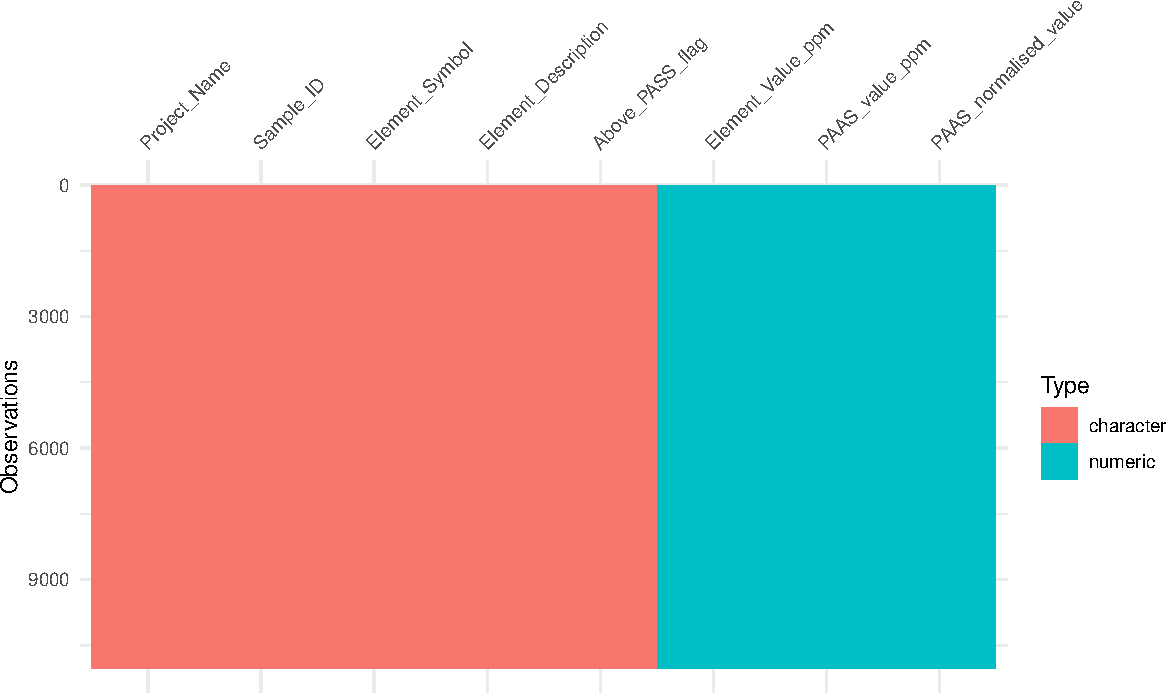
\includegraphics{Final_report_files/figure-latex/visdat-1.pdf}
\caption{\label{fig:visdat}Final Data Wrangling Result}
\end{figure}

\section{Exploratory Data Analysis}\label{exploratory-data-analysis}

The Exploratory Data Analysis (EDA) was carried out on critical elements concentration data, which provide information about the concentration of critical mineral across different areas in Australia that has been normalised using PAAS (Post-Archean Australian Shale) standard. The primary objective of this analysis is to gain a deeper understanding of the data's structure and key characteristics. Through this, we aim to identify significant trends, correlations, and outliers that may influence the outcomes of the study.

The EDA for critical elements concentration data starts with a descriptive statistics for every critical elements included in the data. These summary statistics can be found in the \hyperref[sec-appendixfour]{Appendix 4}. The descriptive statistics features include the minimum value of the critical elements, maximum value, the mean, the median, the standard deviation, and the kurtosis of the variable.

The most important statistics from this table is kurtosis. Kurtosis measures the combined weight of the tails of a distribution relative to its centre. In this way, we can use kurtosis as an indicator of the presence of outliers. A high kurtosis values is indicative of outliers. The summary statistics suggest that Al, Ba, Bi, Ce, Co, Cr, Cs, Cu, Fe, Mn, Nb, and Ni are having many outliers due to high kurtosis value. Validating the outliers will be easier with data visualisation, which will be presented in the next step.

The next step was analysing the distribution of each element's normalised value. By utilising boxplots, it will help identifying the outliers of each critical elements, while also identifying which element's has median value above the PAAS standard. Obtaining these information will help to understand whether certain element is naturally abundance in the nature, thus it is most likely economically efficient to extract. The figure \hyperref[sec-appendixfive]{Appendix 5} provide these informations. The boxplots shows some critical points that can be summarised as follow:

\begin{itemize}
\tightlist
\item
  Medians: Most of the elements have their medians close to 0, indicating that the majority of the values are low or concentrated around a lower range. Considering that the threshold to define whether a sample is below/above background is 1 (vertical red dashed line), some elements that have median above the threshold are Re, Ag, Au, Mo, Bi, Li, Cu, Eu, Dy, Gd, Sm, Lu, Yb, Tm, Tb, MREEs, Er, Ho, U, Ga, Y, Pb, Nd, Sc, REEYs, REEs, Th, V, Pr, LREEs.
\item
  Spread and variability: The elements exhibit varying degrees of spread. For example, Ge shows a wide range with its box stretching from a low value near 0 to a higher value around 10, indicating a large variability. On the opposite side, elements like Mn, Fe, Cr, Co, Rb, Ni, HREEs have very narrow IQR, indicating less variability.
\item
  Outliers: Several elements have significant outliers, as indicated by the dots outside the whiskers of the box plots. For instance, Ge, Bi, Mn, and Ba show notable outliers far from the main data range. Additionally, some elements that was reported from \hyperref[sec-appendixfive]{Appendix 5}, which have high kurtosis are Al, Ba, Bi, Ce, Co, Cr, Cs, Cu, Fe, Mn, Nb, and Ni. These outliers suggest the presence of some unusually high or low values for these elements, which could be of interest for further investigation.
\item
  Symmetry and skewness: Some elements like Ge, Bi, and Ag appear to have a right skew, with longer whiskers or outliers extending to the right, indicating that the distribution of their normalised values has a tail on the higher end. Elements like Ga and Sm show a more symmetrical distribution with whiskers extending fairly equally on both sides of the box.
\item
  Comparison across Elements: Ge stands out with a particularly large spread and median, making it an outliers among the elements. Conversely, many rare earth elements (REEs, REEYs, MREEs, LREEs, HREEs) have relatively low medians and a small spread, indicating that their normalised values are generally low and clustered.
\end{itemize}

\subsection{Predictive Modelling}\label{predictive-modelling}

While some general EDA has been conducted, a more in-depth analysis specific to predictive modeling is required. As mentioned earlier, the predictive models will use only the 11 elements tested in the ME-4ACD1 analysis. This section will therefore focus exclusively on those elements.

Table \ref{tab:descstatsflt} shows the descriptive statistics of the dependent variables (REEs, HREEs, and LREEs) and independent variables (all elements from ME-4ACD1 test).

\begin{table}[!h]
\centering
\caption{\label{tab:descstatsflt}\textbf{Descriptive Statistics of Dependent and Independent Variables}}
\centering
\fontsize{10}{12}\selectfont
\begin{tabu} to \linewidth {>{\centering}X>{\centering}X>{\centering}X>{\centering}X>{\centering}X>{\centering}X>{\centering}X}
\toprule
Element Symbol & Min & Max & Mean & Median & SD & Kurtosis\\
\midrule
\cellcolor{gray!10}{Ag} & \cellcolor{gray!10}{0.10} & \cellcolor{gray!10}{0.66} & \cellcolor{gray!10}{0.21} & \cellcolor{gray!10}{0.18} & \cellcolor{gray!10}{0.12} & \cellcolor{gray!10}{5.78}\\
\addlinespace
Cd & 0.01 & 0.72 & 0.12 & 0.09 & 0.11 & 9.84\\
\addlinespace
\cellcolor{gray!10}{Co} & \cellcolor{gray!10}{2.00} & \cellcolor{gray!10}{134.00} & \cellcolor{gray!10}{15.40} & \cellcolor{gray!10}{10.00} & \cellcolor{gray!10}{19.27} & \cellcolor{gray!10}{17.66}\\
\addlinespace
Cu & 1.00 & 255.00 & 42.02 & 47.00 & 28.99 & 13.14\\
\addlinespace
\cellcolor{gray!10}{HREE} & \cellcolor{gray!10}{1.10} & \cellcolor{gray!10}{30.60} & \cellcolor{gray!10}{8.67} & \cellcolor{gray!10}{8.20} & \cellcolor{gray!10}{4.81} & \cellcolor{gray!10}{6.71}\\
\addlinespace
LREE & 11.70 & 554.50 & 134.28 & 140.06 & 71.05 & 6.99\\
\addlinespace
\cellcolor{gray!10}{Li} & \cellcolor{gray!10}{5.00} & \cellcolor{gray!10}{285.00} & \cellcolor{gray!10}{47.72} & \cellcolor{gray!10}{40.00} & \cellcolor{gray!10}{39.49} & \cellcolor{gray!10}{9.53}\\
\addlinespace
Mo & 0.10 & 20.60 & 4.46 & 4.00 & 3.29 & 10.24\\
\addlinespace
\cellcolor{gray!10}{Ni} & \cellcolor{gray!10}{1.00} & \cellcolor{gray!10}{360.00} & \cellcolor{gray!10}{16.97} & \cellcolor{gray!10}{7.00} & \cellcolor{gray!10}{38.25} & \cellcolor{gray!10}{44.10}\\
\addlinespace
Pb & 0.89 & 83.45 & 21.69 & 21.00 & 14.54 & 6.14\\
\addlinespace
\cellcolor{gray!10}{REE} & \cellcolor{gray!10}{19.60} & \cellcolor{gray!10}{611.00} & \cellcolor{gray!10}{159.33} & \cellcolor{gray!10}{165.43} & \cellcolor{gray!10}{78.89} & \cellcolor{gray!10}{6.57}\\
\addlinespace
Sc & 2.20 & 67.80 & 15.47 & 16.20 & 8.30 & 8.48\\
\addlinespace
\cellcolor{gray!10}{Tl} & \cellcolor{gray!10}{0.03} & \cellcolor{gray!10}{10.00} & \cellcolor{gray!10}{1.94} & \cellcolor{gray!10}{0.72} & \cellcolor{gray!10}{3.12} & \cellcolor{gray!10}{5.78}\\
\addlinespace
Zn & 1.00 & 307.00 & 65.38 & 66.00 & 49.65 & 4.13\\
\bottomrule
\end{tabu}
\end{table}

Figure \ref{fig:bpflt} shows the distribution of all 11 elements. The analysis has been conducted in the previous section. However, to emphasise the point, it is clear that the distribution of all elements are not balance (do not follow normal distribution), with many outliers that might affect the model performance later. A further data processing might be needed to reduce the effect of these outliers value in the model construction.

\begin{figure}

{\centering 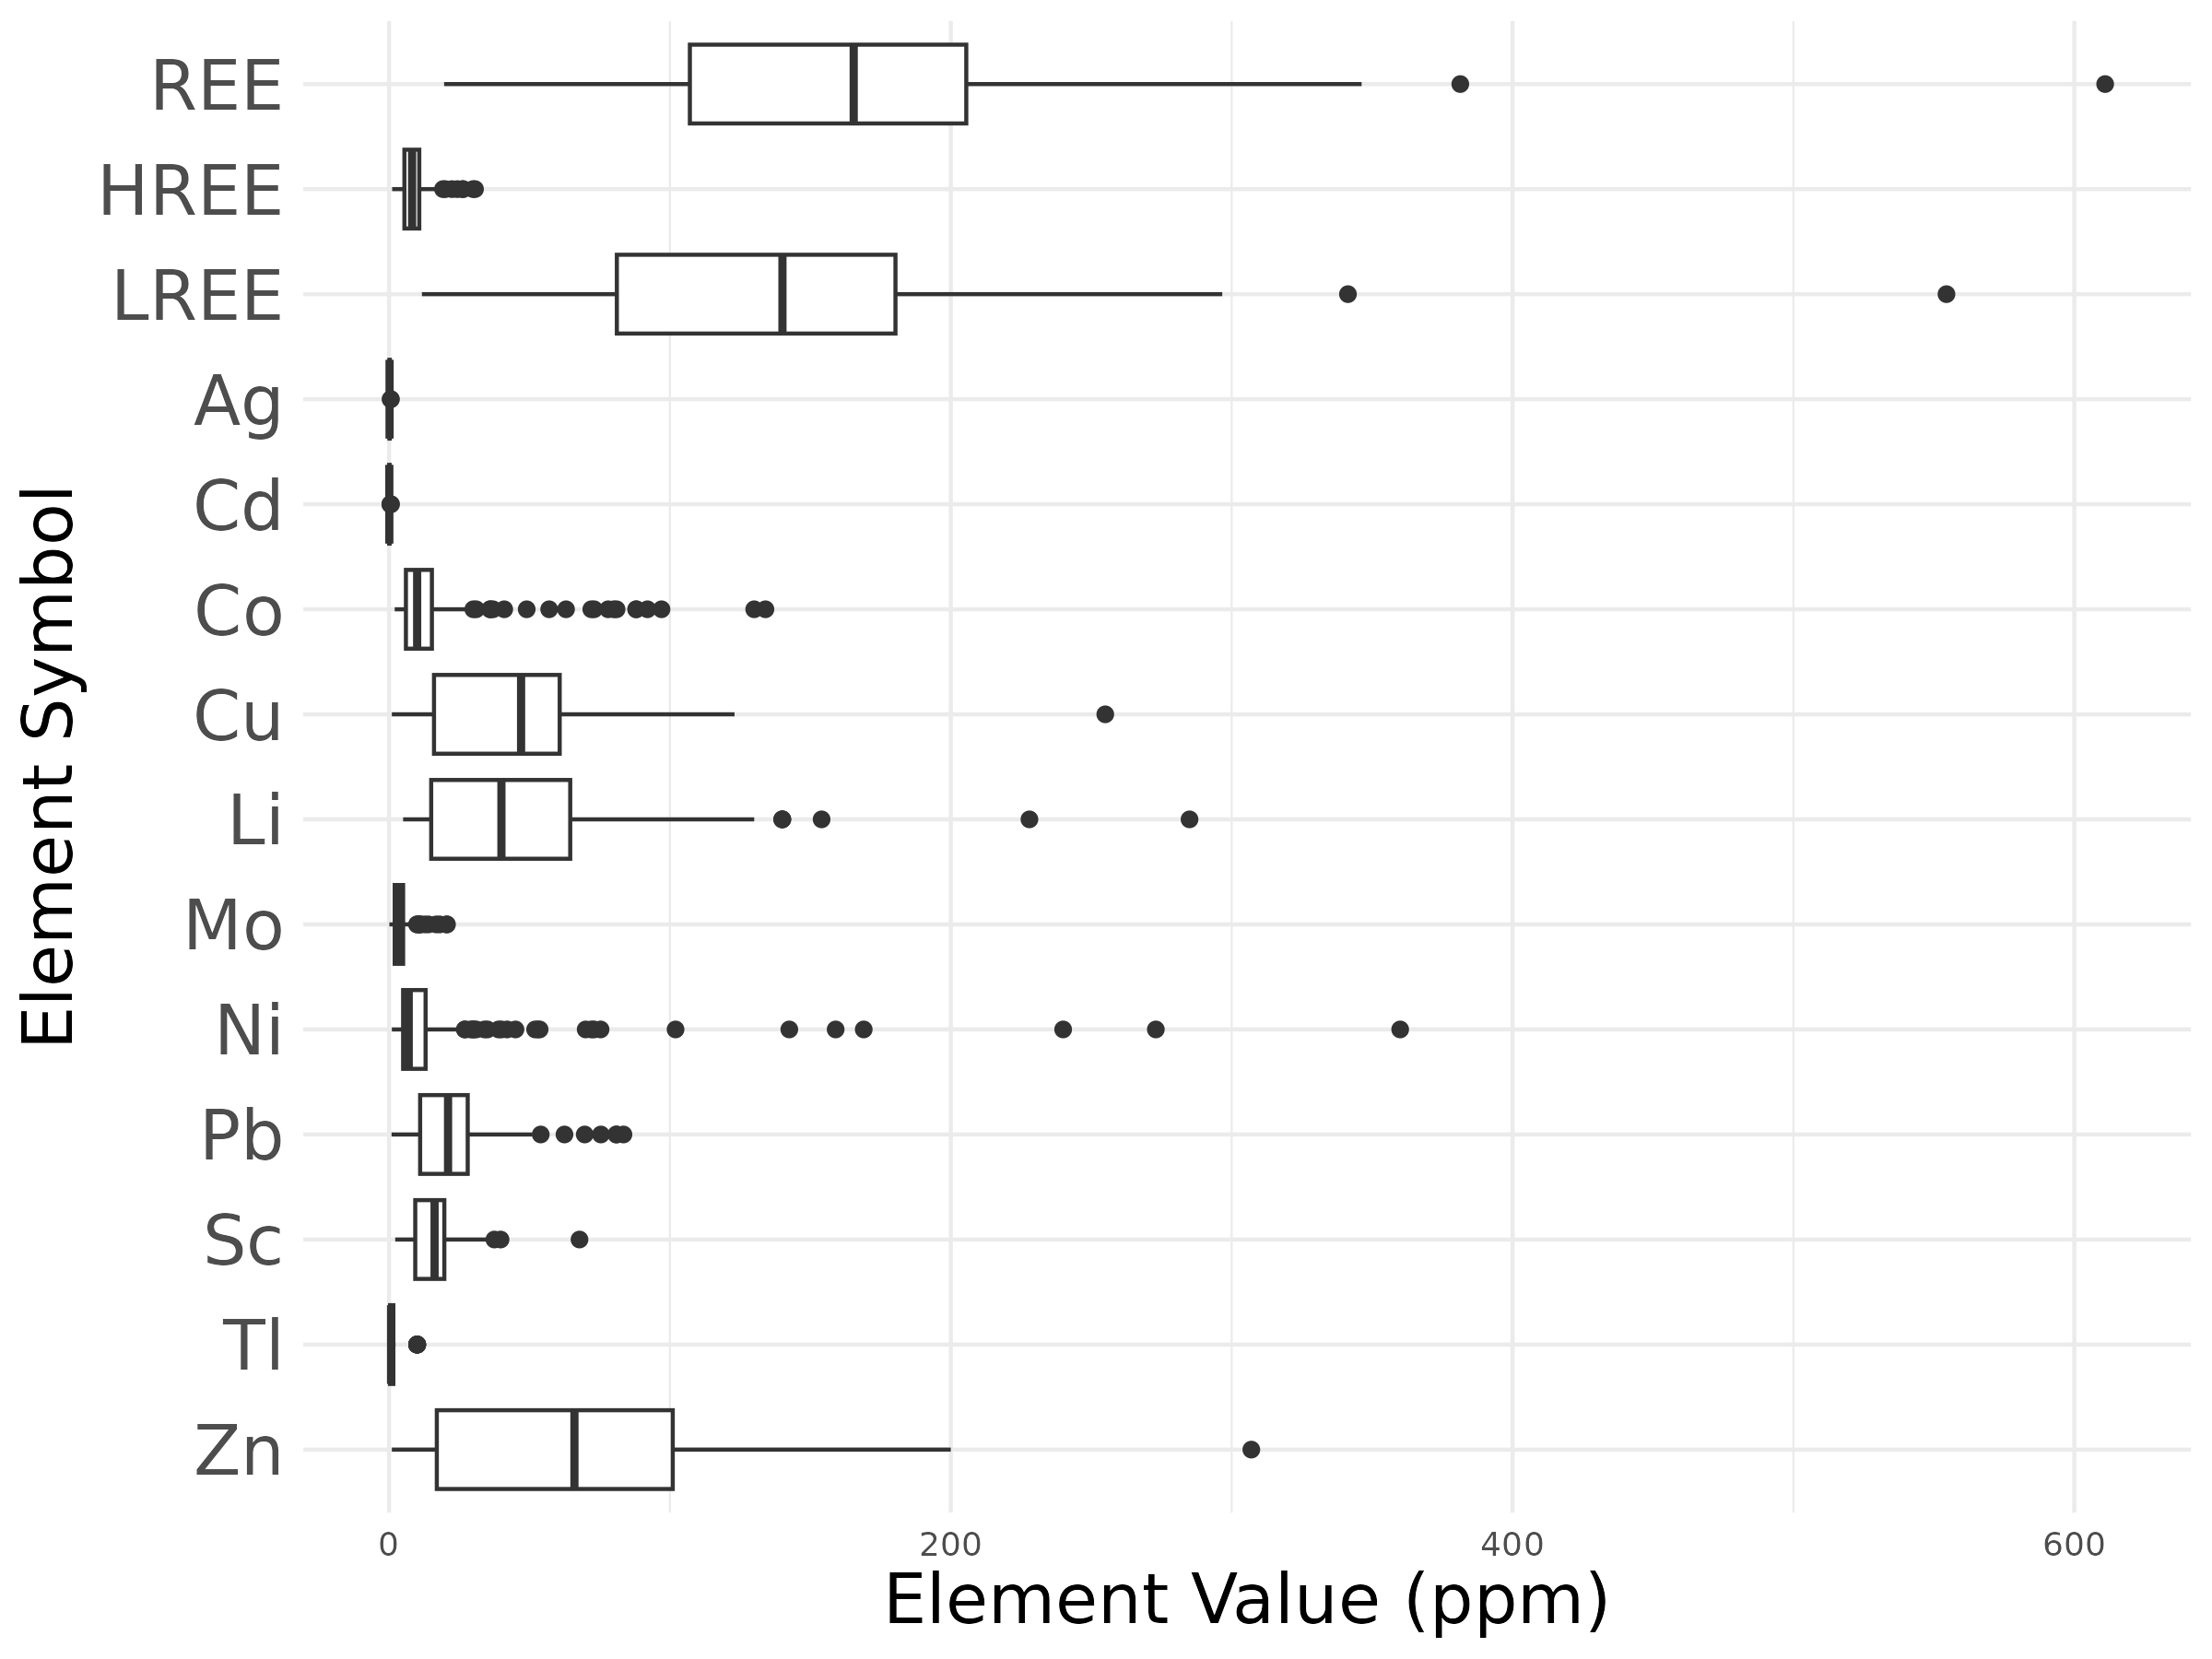
\includegraphics[width=1\linewidth,height=0.3\textheight]{Final_report_files/figure-latex/bp_test_a} 

}

\caption{The Box Plot of Dependent and Independent Variables for Predictive Modelling}\label{fig:bpflt}
\end{figure}

Figure \ref{fig:corrmat} shows the correlation matrix of all elements, the main interesting information from this matrix is to understand the correlation coefficient of the dependent and independent variables. As can be seen, in overall there is no significant correlation coefficient between the dependent variables and independent variables, with the highest is only moderately strong (0.68 between Pb and LREEs). This poses a potential challenge in predicting the dependent variable later in the predictive modelling.

\begin{figure}

{\centering 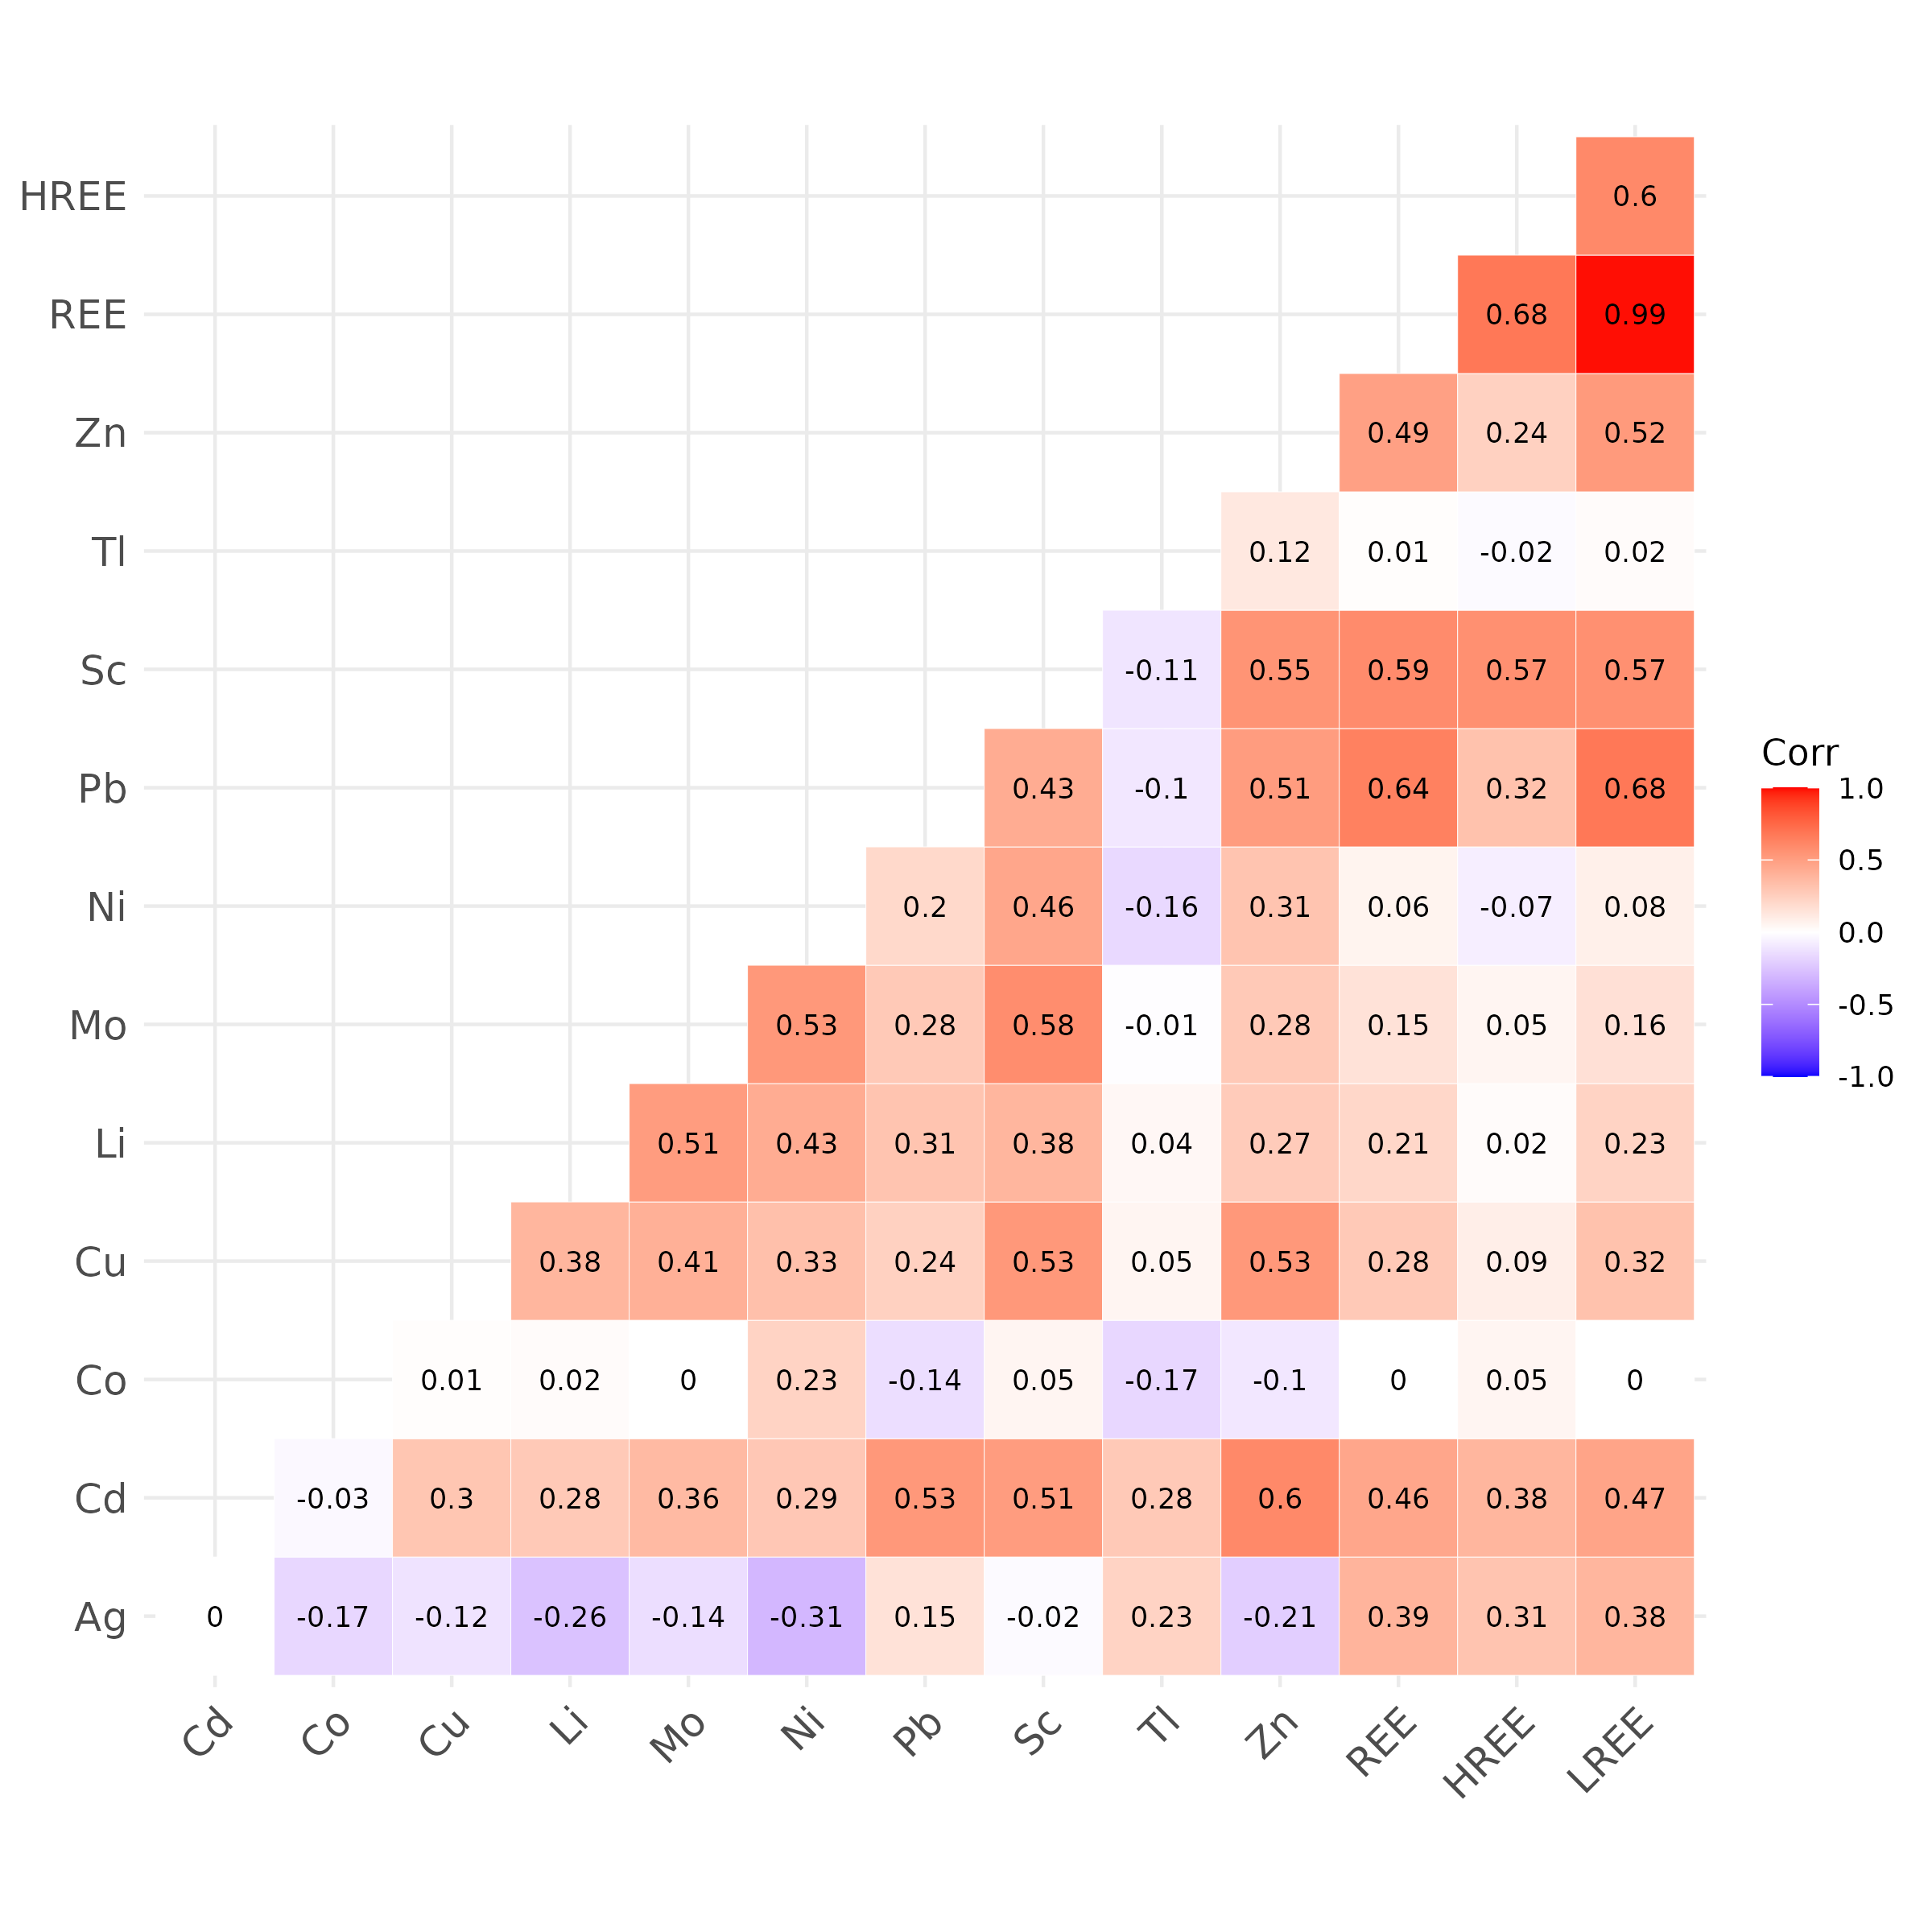
\includegraphics[width=1\linewidth,height=0.45\textheight]{Final_report_files/figure-latex/pg_cop_cheaper} 

}

\caption{Correlation Matrix of All Variables}\label{fig:corrmat}
\end{figure}

\newpage

\section{Methodology}\label{methodology}

\subsection{Predictive Modelling}\label{predictive-modelling-1}

\begin{figure}

{\centering 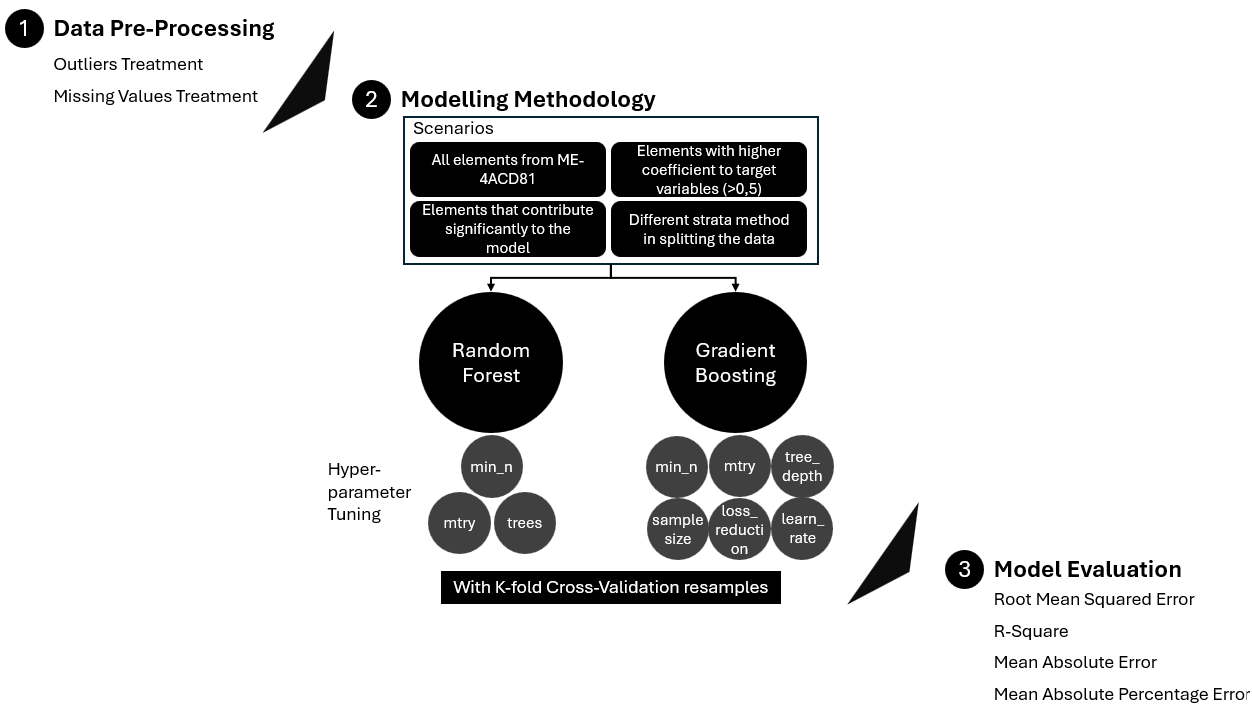
\includegraphics[width=0.95\linewidth]{Final_report_files/figure-latex/Methodologyv2} 

}

\caption{The Methodology of This Study}\label{fig:modelbuilding}
\end{figure}

The predictive modeling process in this study follows a structured methodology, consisting of key steps aimed at selecting the most accurate and robust model for predicting the target variable. Each step contributes to refining the model's performance, from data pre-processing and feature selection to model training and evaluation. The framework of this methodology is shown in the figure \ref{fig:modelbuilding}.

The methodology for this study follows a three-stage process. First, further data pre-processing is conducted, addressing outliers and missing values to ensure clean data. Next, several modeling scenarios are explored using Random Forest and Gradient Boosting, with hyperparameter tuning applied to optimise model performance. These scenarios include using all elements, elements with high correlation coefficient to target variables, and different stratification methods for data splitting. Finally, model performance is evaluated using key metrics such as Root Mean Squared Error (RMSE), R-squared, Mean Absolute Error (MAE), and Mean Absolute Percentage Error (MAPE).

\subsubsection{Data Pre-Processing}\label{data-pre-processing}

On one hand, outliers is well known as the observations/data points that deviate significantly from other observations in a dataset. On the other hand, missing value is observation when there is no data stored for certain variables. In predictive modelling, outliers and missing value can have an effect to the regression model when predicting the target variable in a negative way. For example, outliers value will disrupt the normal pattern of the dataset, while missing value will introduce uncertainty to the model. Thus, if not treated, they might lead the model to make inaccurate predictions. With this concern, outliers and missing value will be treated, aimed to reduce the negative effect to the model performance \autocite{Hastie09}.

For outliers, \textcite{tukey1977} introduce the approach to detect outliers in a dataset. He defined that outliers can be detected by the 1.5 Interquartile Range (IQR). An observation is considered an outliers if it lies below Q1 - 1.5xIQR or above Q3 + 1.5xIQR, where IQR is the interquartile range between the first and third quartiles. This method is particularly effective for detecting outliers in data with a skewed distribution, align with the skewed distribution from the distribution analysis. It will be applied to the dataset for this study in detecting outliers. Next, in treating the outliers, \autocite{Barnett1995} stated that, as a simple approach, outliers can be replaced with sample median for robust estimation. This will also reduce the weight of incorrect value which was inputted during the lab test. The outliers will be replaced with median value of where the samples were obtained from. For example, for outliers detected in ``Sc'' data from ``Confidential Project A'', will be replaced with median value of ``Sc'' of ``Confidential Project A''.

For missing values, \textcite{Hastie09} stated that there are number of ways in treating missing value (assuming random missing value), which are removing observations with any missing value; rely on the learning algorithm to handle missing values during the training process; and fill in all missing values prior to training process. The last option was chosen and the missing value are filled with the median value of where the samples were obtained from, but if the element does not exist in that particular project, then the global median will be applied. For example, for missing value detected in ``Sc'' data from ``Confidential Project A'', then those missing values will be replaced with median value of ``Sc'' in general.

Finally, after treating outliers and missing values, the processed data will be split with a 2/3 proportion for training and 1/3 for testing follows a widely accepted practice in predictive modelling. This approach ensures robust evaluation of model's performance on unseen case, which helps avoid overfitting. Stratifying by project area was essential to account for the inherent variability across different mining sites. Since element's concentration values vary significantly by location, stratification ensures that the training and testing datasets maintain a representative distribution of project areas.

\subsubsection{Prediction Model}\label{prediction-model}

In this project, the tidymodels package will be used to implement predictive modeling in R. Tidymodels is a comprehensive framework built on tidyverse principles, designed for modeling and machine learning \autocite{tidymodels}. In addition, two prediction methods are employed in this analysis: Random Forest (RF) and Gradient Boosting Tree (GBT), both of which are well-suited for handling complex, non-linear relationships in the data. These methods have been selected for their robustness in prediction and their ability to minimise overfitting through ensemble learning techniques.

Random Forest is an ensemble learning method that constructs multiple decision trees using subsets of the training data through a technique called `bagging' (Bootstrap Aggregating). Bagging is a variance reduction technique for an estimated prediction function. In regression, this involves fitting the same regression tree multiple times to different bootstrap samples of the training data and averaging the results. Random Forest is a significant modification of bagging, as it builds a large collection of de-correlated trees and then averages their outputs. The concept behind Random Forest is to improve the variance reduction achieved by bagging by reducing the correlation between the trees, while minimizing any increase in variance. This is accomplished by randomly selecting input variables during the tree-growing process \autocite{Hastie09,Breiman01}. The engine setting in tidymodels will be set to \texttt{randomForest}.

Whereas random forests build an ensemble of deep independent trees, GBT build an ensemble of shallow trees in sequence with each tree learning and improving on the previous one. The main idea of boosting is to add new models to the ensemble sequentially. In essence, boosting attacks the bias-variance-trade off by starting with a weak model (e.g., a decision tree with only a few splits) and sequentially boosts its performance by continuing to build new trees, where each new tree in the sequence tries to fix up where the previous one made the biggest mistakes (i.e., each new tree in the sequence will focus on the training rows where the previous tree had the largest prediction errors) \autocite{boehmke2019}. The engine setting in tidymodels will be set to \texttt{xgboost}.

\subsubsection{Hyperparameter tuning}\label{hyperparameter-tuning}

Building an effective machine learning model is a complex and time-intensive process that requires selecting the appropriate algorithm and optimising the model's architecture through hyperparameter tuning. Machine learning models have two kinds of parameters: model parameters, which are initialised and updated during the training process (such as weights in neural networks), and hyperparameters, which cannot be learned from the data and must be set before training begins. Hyperparameters define key aspects of the model's structure and learning process. Examples include the penalty parameter in support vector machines, the learning rate in neural networks, the activation function, and optimiser types. Hyperparameter tuning is essential for improving model performance, as it involves finding the optimal combination of settings that maximises predictive accuracy \autocite{YANG2020295}. Tree-based model have more hyperparameter that can be tuned, however, for this project, seven key hyperparameters were the top priority for tuning, which are:

1). \texttt{mtry} (number of predictors to sample): Controls the number of predictors considered at each split in a decision tree. A smaller mtry introduces more variability among trees, while a larger mtry can lead to more accurate splits but risks in overfitting problem.

2). \texttt{min\_n} (minimal terminal node size): Determines the minimum number of observations in the ending node. Smaller values allow trees to grow deeper, capturing more details in training data, while larger values lead to simpler models that may generalize better.

3). \texttt{trees} (number of trees): Define the the total number of decision trees in the ensemble. More trees generally improve performance but also increase computational cost.

4). \texttt{tree\_depth} (tree depth): Controls the depth of the individual trees.

5). \texttt{learn\_rate} (learning rate): It determines the influence of each tree on the final prediction and regulates the pace at which the algorithm progresses along the gradient descent path (or learns).

6). \texttt{sample\_size} (sample size): Define the the total number of decision trees in the ensemble. More trees generally improve performance but also increase computational cost.

7). \texttt{loss\_reduction} (minimum loss reduction): The reduction in the loss function required to split further

To determine the best combination of these hyperparameters in the grid, \emph{k}-fold cross-validation was applied. In k-fold cross-validation, the dataset is randomly divided into \emph{k} equal-sized groups, known as ``folds.'' For each resampling iteration, the model is trained on \emph{k}-1 folds, while the remaining fold is used for validation. In standard \emph{k}-fold cross-validation (without repetition), the process is repeated \emph{k} times, ensuring that each fold is used once for validation \autocite{tidymodels}. Cross-validation provides a reliable estimate of the optimal tuning parameter value.

\subsubsection{Model evaluation}\label{model-evaluation}

When assessing a model's performance on a particular dataset, it is essential to have a method for determining how closely its predictions align with the actual observed data. This involves measuring the degree to which the predicted value for an observation approximates the true value for that observation. In this project, several metrics will be used, including Root Mean Squared Error (RMSE), Mean Absolute Error (MAE), Mean Absolute Percentage Error (MAPE), and R-Squared. These metrics provide a comprehensive understanding of how well the model fits the data, capturing both the average magnitude of error and the variability explained by the model \autocite{ISLR,Hastie09}.

\paragraph{Root Mean Squared Error (RMSE)}\label{root-mean-squared-error-rmse}

RMSE is a standard way to measure the error of a model in predicting continuous outcomes. It represents the square root of the average of the squared differences between the observed and predicted values. RMSE gives more weight to large errors, making it particularly useful when large errors are undesirable \autocite{ISLR,Hastie09}. The formula for RMSE is:

\[RMSE = \sqrt{\frac{1}{n} {\sum^n_{i=1}(y_i-\hat{y_i})^2}}\]

where \(y_i\) is the actual value, \(\hat{y_i}\) is the predicted value, and n is the number of observations.

\paragraph{Mean Absolute Error (MAE)}\label{mean-absolute-error-mae}

MAE measures the average magnitude of the errors in a set of predictions, without considering their direction. It's a linear score, meaning all individual differences are weighted equally \autocite{ISLR,Hastie09}. The formula for MAE is:

\[MAE = \frac{1}{n} {\sum^n_{i=1}|y_i-\hat{y_i}|}\]

MAE is easy to interpret because it provides the average error in the same units as the target variable.

\paragraph{Mean Absolute Percentage Error (MAPE)}\label{mean-absolute-percentage-error-mape}

MAPE expresses the error as a percentage of the actual values, making it useful for comparing models on different scales or datasets. However, MAPE can be problematic when actual values are very close to zero \autocite{ISLR,Hastie09}. The formula for MAPE is:

\[MAPE = \frac{100\%}{n} {\sum^n_{i=1}|\frac{y_i-\hat{y_i}}{y_i}|}\]

\paragraph{R-squared (Coefficient of Determination)}\label{r-squared-coefficient-of-determination}

R-squared explains the proportion of the variance in the dependent variable that is predictable from the independent variables. It provides insight into how well the model captures the variability in the data, with a higher R-squared indicating a better fit \autocite{ISLR,Hastie09}. The formula for R-squared is:

\[R^2 = 1-\frac{\sum^n_{i=1}(y_i-\hat{y_i})^2}{\sum^n_{i=1}(y_i-\bar{y})^2}\]

where \(\bar{y}\) is the mean of the actual values.

\paragraph{Additional Considerations}\label{additional-considerations}

These evaluation metrics each have strengths and weaknesses. RMSE penalises large errors more than MAE, making it more sensitive to outliers. MAPE is useful for interpretation as it gives a percentage error, but it can be misleading when actual values are very low. R-squared is a useful measure of fit, but it can sometimes be artificially high in overfitting scenarios. Therefore, it is essential to use a combination of these metrics to gain a well-rounded understanding of the model's performance. For this project, we are going to look for a model that produce the smallest RMSE, MAE, and MAPE, while produce the largest R-Squared, because this implies the model produce the least error and cover the most variability from the data.

\subsubsection{Model Scenarios}\label{model-scenarios}

To build the predictive models, several scenarios were tested to determine which combination of elements provides the best performance in predicting REEs, HREEs, and LREEs. First, a model will be constructed using all elements from ME-4ACD81 test. Second, variable importance will be analysed to identify which variable contribute most to the prediction model, and these will be used in constructing to construct the second model. Third, elements with a high correlation coefficient (above 0.5) will be used to build another model. Among these three scenarios, the one that produces the best result will be applied using the GBT method to evaluate potential improvement with different machine learning techniques.

\subsection{Enrichment Analysis}\label{enrichment-analysis}

PAAS (Post-Archean Australian Average Shale) represents the precise composition of the upper crust, which is derived from the average of 23 shales in Post-Archean age, with the exclusion of aberrant materials and the correction of quadratic equation. \textcite{McLennan1989} stated that PAAS normalisation refers to the process of tested element concentrations normalisation against the PAAS score, providing a standardised way to element abundance across different samples. The The formula can be written as

\[\text{PAAS Normalized}=\frac{ \text{Element Concentration in Sample (ppm)}}{\text{PAAS Concentration (ppm)}}\]

The cut-off benchmark is 1 ppm for the classification of element enrichment. A ratio exceeding 1 ppm indicates that the element concentration in the sample is enriched relative to PAAS standard, implying potential for economic extraction, vice versa.

The visualisation technique adopts the distribution scatter plot for two scenarios: 1). Aggregating all testing samples in global project to comprehend which element is considered enrichment from a holistic perspective and 2). Splitting down to each individual project to identify which region is relatively enriched than others.

\newpage

\section{Results}\label{results}

\subsection{Predictive Modelling}\label{predictive-modelling-2}

\begin{table}[!h]
\centering
\caption{\label{tab:testres1}\textbf{Evaluation Metrics for Predicting REE Across Different Scenarios}}
\centering
\fontsize{10}{12}\selectfont
\begin{tabu} to \linewidth {>{\centering\arraybackslash}p{1,2cm}>{\raggedright\arraybackslash}p{1cm}>{\raggedright\arraybackslash}p{4,5cm}>{\raggedright\arraybackslash}p{3,1cm}>{\centering}X>{\centering}X>{\centering}X>{\centering}X}
\toprule
Target Variable & Method & Scenarios & Elements & RMSE & MAE & MAPE & R Squared\\
\midrule
\cellcolor{gray!10}{REE} & \cellcolor{gray!10}{Random Forest} & \cellcolor{gray!10}{Elements with correlation coefficient above 0.5} & \cellcolor{gray!10}{Pb, Sc} & \cellcolor{gray!10}{55.65} & \cellcolor{gray!10}{38.04} & \cellcolor{gray!10}{0.29} & \cellcolor{gray!10}{0.48}\\
\addlinespace
REE & Random Forest & Default tuned & All elements & 47.57 & 33.85 & 0.26 & 0.62\\
\addlinespace
\cellcolor{gray!10}{REE} & \cellcolor{gray!10}{Random Forest} & \cellcolor{gray!10}{Elements with high variable importance} & \cellcolor{gray!10}{Pb, Tl, Sc, Zn, Cu, Cd} & \cellcolor{gray!10}{48.82} & \cellcolor{gray!10}{35.76} & \cellcolor{gray!10}{0.28} & \cellcolor{gray!10}{0.60}\\
\addlinespace
REE & XGBoost & Default tuned & All elements & 50.37 & 37.26 & 0.29 & 0.57\\
\bottomrule
\end{tabu}
\end{table}

Table \ref{tab:testres1} shows the model performance evaluation for predicting REE, HREE, and LREE across different scenarios. For REE prediction, the predictive model was built under four different scenarios. From the error evaluation metrics, the RMSE value is ranging from 47.57 to 55.65, MAE value is ranging from 33.85 to 38.04, and MAPE value is ranging from 26.40\% to 29.44\%. A model with the lowest value indicates the least error, which turn out the random forest default tuned model where all elements are included is the lowest of all. Additionally, from the variability metric, the R-Square value is ranging from 0.48 to 0.62. A model with the highest value indicates a better model in capturing variability of the data, in this case the same model also score the the highest of all. This results concludes the best model in predicting REE is the random forest default tuned model where all elements are included.

\begin{table}[!h]
\centering
\caption{\label{tab:testres2}\textbf{Evaluation Metrics for Predicting HREE Across Different Scenarios}}
\centering
\fontsize{10}{12}\selectfont
\begin{tabu} to \linewidth {>{\centering\arraybackslash}p{1,2cm}>{\raggedright\arraybackslash}p{1cm}>{\raggedright\arraybackslash}p{4,5cm}>{\raggedright\arraybackslash}p{3,1cm}>{\centering}X>{\centering}X>{\centering}X>{\centering}X}
\toprule
Target Variable & Method & Scenarios & Elements & RMSE & MAE & MAPE & R Squared\\
\midrule
\cellcolor{gray!10}{HREE} & \cellcolor{gray!10}{Random Forest} & \cellcolor{gray!10}{Default tuned} & \cellcolor{gray!10}{All elements} & \cellcolor{gray!10}{3.33} & \cellcolor{gray!10}{2.13} & \cellcolor{gray!10}{0.29} & \cellcolor{gray!10}{0.46}\\
\addlinespace
HREE & Random Forest & Model with high variable importance & Pb, Sc & 3.60 & 2.48 & 0.37 & 0.37\\
\addlinespace
\cellcolor{gray!10}{HREE} & \cellcolor{gray!10}{XGBoost} & \cellcolor{gray!10}{Model with high variable importance} & \cellcolor{gray!10}{Pb, Sc} & \cellcolor{gray!10}{3.55} & \cellcolor{gray!10}{2.36} & \cellcolor{gray!10}{0.34} & \cellcolor{gray!10}{0.39}\\
\bottomrule
\end{tabu}
\end{table}

For HREE prediction, the predictive model was built under three different scenarios, shown in Table \ref{tab:testres2}. A scenario where we construct the model with elements which has correlation coefficient above 0.5 is absent because there is only one element that fall under this category (Sc). It was decided not to perform this scenario for HREE for the reason that Sc correlation coefficient to HREE is only 0.57, with just moderately strong coefficient, authors thought predicting HREE with one element will: first, oversimplified the model; second, ignore the fact that HREE is less abundant in the nature which further reduces the likelihood that a single moderately correlated element could serve as a reliable predictor. Next, From the error evaluation metrics, the RMSE value is ranging from 3.33 to 3.60, MAE value is ranging from 2.13 to 2.48, and MAPE value is ranging from 29\% to 37\%. The default model with all elements included has the lowest value of RMSE, MAE, and MAPE. Moreover, R-Square value is ranging from 0.37 to 0.46. In this case, the default model has the highest score as well. In Overall, it is clear that the default model which constructed by having all elements from ME-4ACD81 test is the best model in predicting HREE.

\begin{table}[!h]
\centering
\caption{\label{tab:testres3}\textbf{Evaluation Metrics for Predicting LREE Across Different Scenarios}}
\centering
\fontsize{10}{12}\selectfont
\begin{tabu} to \linewidth {>{\centering\arraybackslash}p{1,2cm}>{\raggedright\arraybackslash}p{1cm}>{\raggedright\arraybackslash}p{4,5cm}>{\raggedright\arraybackslash}p{3,1cm}>{\centering}X>{\centering}X>{\centering}X>{\centering}X}
\toprule
Target Variable & Method & Scenarios & Elements & RMSE & MAE & MAPE & R Squared\\
\midrule
\cellcolor{gray!10}{LREE} & \cellcolor{gray!10}{Random Forest} & \cellcolor{gray!10}{Default tuned} & \cellcolor{gray!10}{All elements} & \cellcolor{gray!10}{39.61} & \cellcolor{gray!10}{26.62} & \cellcolor{gray!10}{0.25} & \cellcolor{gray!10}{0.61}\\
\addlinespace
LREE & Random Forest & Elements with high variable importance & Tl, Pb, Sc, Cd, Zn, Cu & 40.48 & 27.71 & 0.27 & 0.59\\
\addlinespace
\cellcolor{gray!10}{LREE} & \cellcolor{gray!10}{Random Forest} & \cellcolor{gray!10}{Elements with correlation coefficient above 0.5} & \cellcolor{gray!10}{Pb, Sc, Zn} & \cellcolor{gray!10}{38.44} & \cellcolor{gray!10}{29.60} & \cellcolor{gray!10}{0.31} & \cellcolor{gray!10}{0.63}\\
\addlinespace
LREE & XGBoost & Elements with correlation coefficient above 0.5 & Pb, Sc, Zn & 41.71 & 31.08 & 0.27 & 0.57\\
\bottomrule
\end{tabu}
\end{table}

Table \ref{tab:testres3} shows the results for LREE prediction, where four different scenarios was performed. From the error evaluation metrics, the RMSE value is ranging from 38.44 to 41.71, MAE value is ranging from 26.62 to 31.08, and MAPE value is ranging from 25.07\% to 31.38\%. The model that was constructed using elements with correlation coefficient above 0.5 score the lowest of all, making it the model with least error rate. Furthermore, R-Square value is ranging from 0.57 to 0.63. In this case, the same model score the highest. It can be concluded that the random forest which constructed with elements that has correlation coefficient value above 0.5 is the best model in predicting LREE.

With the best model identified, figure \ref{fig:bestplot} shows the predicted vs actual values of each model. The red dashed diagonal line portray the ideal scenario where the predicted values perfectly match the actual values. Points lying on this line indicate perfect prediction, while deviations from the line reflect prediction errors.

\begin{figure}

{\centering 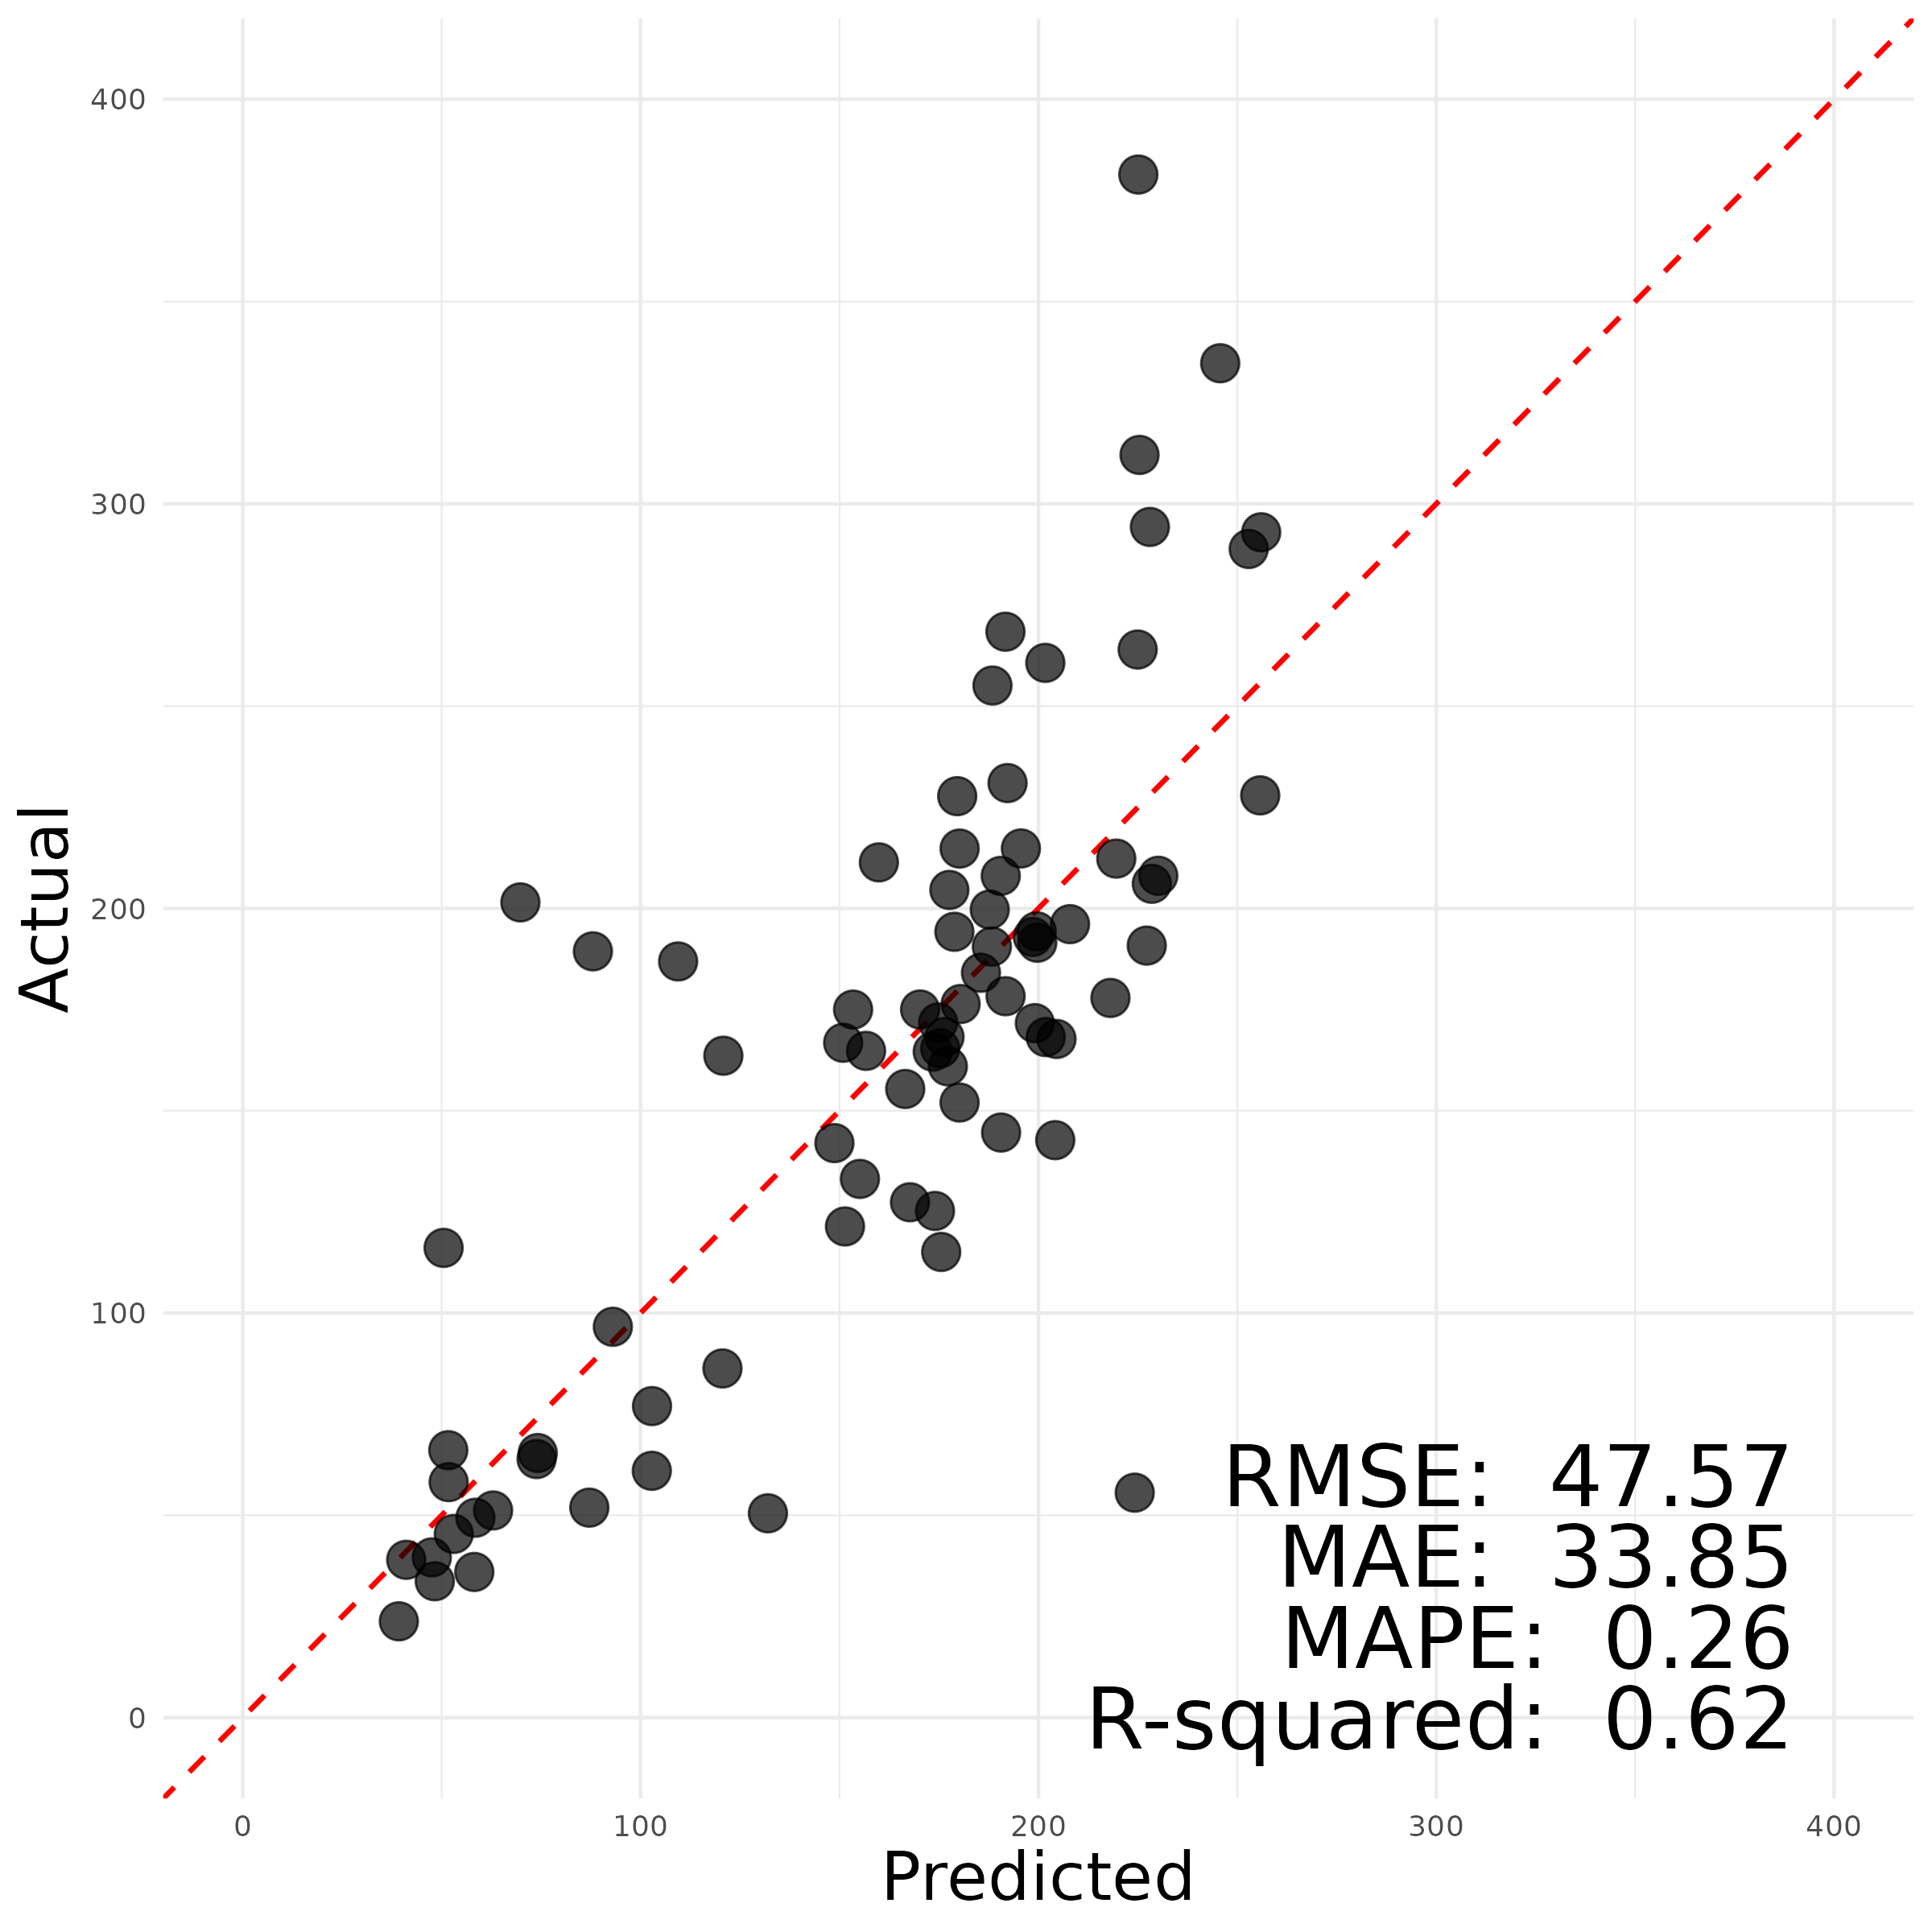
\includegraphics[width=0.3\linewidth,height=0.4\textheight]{Final_report_files/figure-latex/results_ree_test_best} 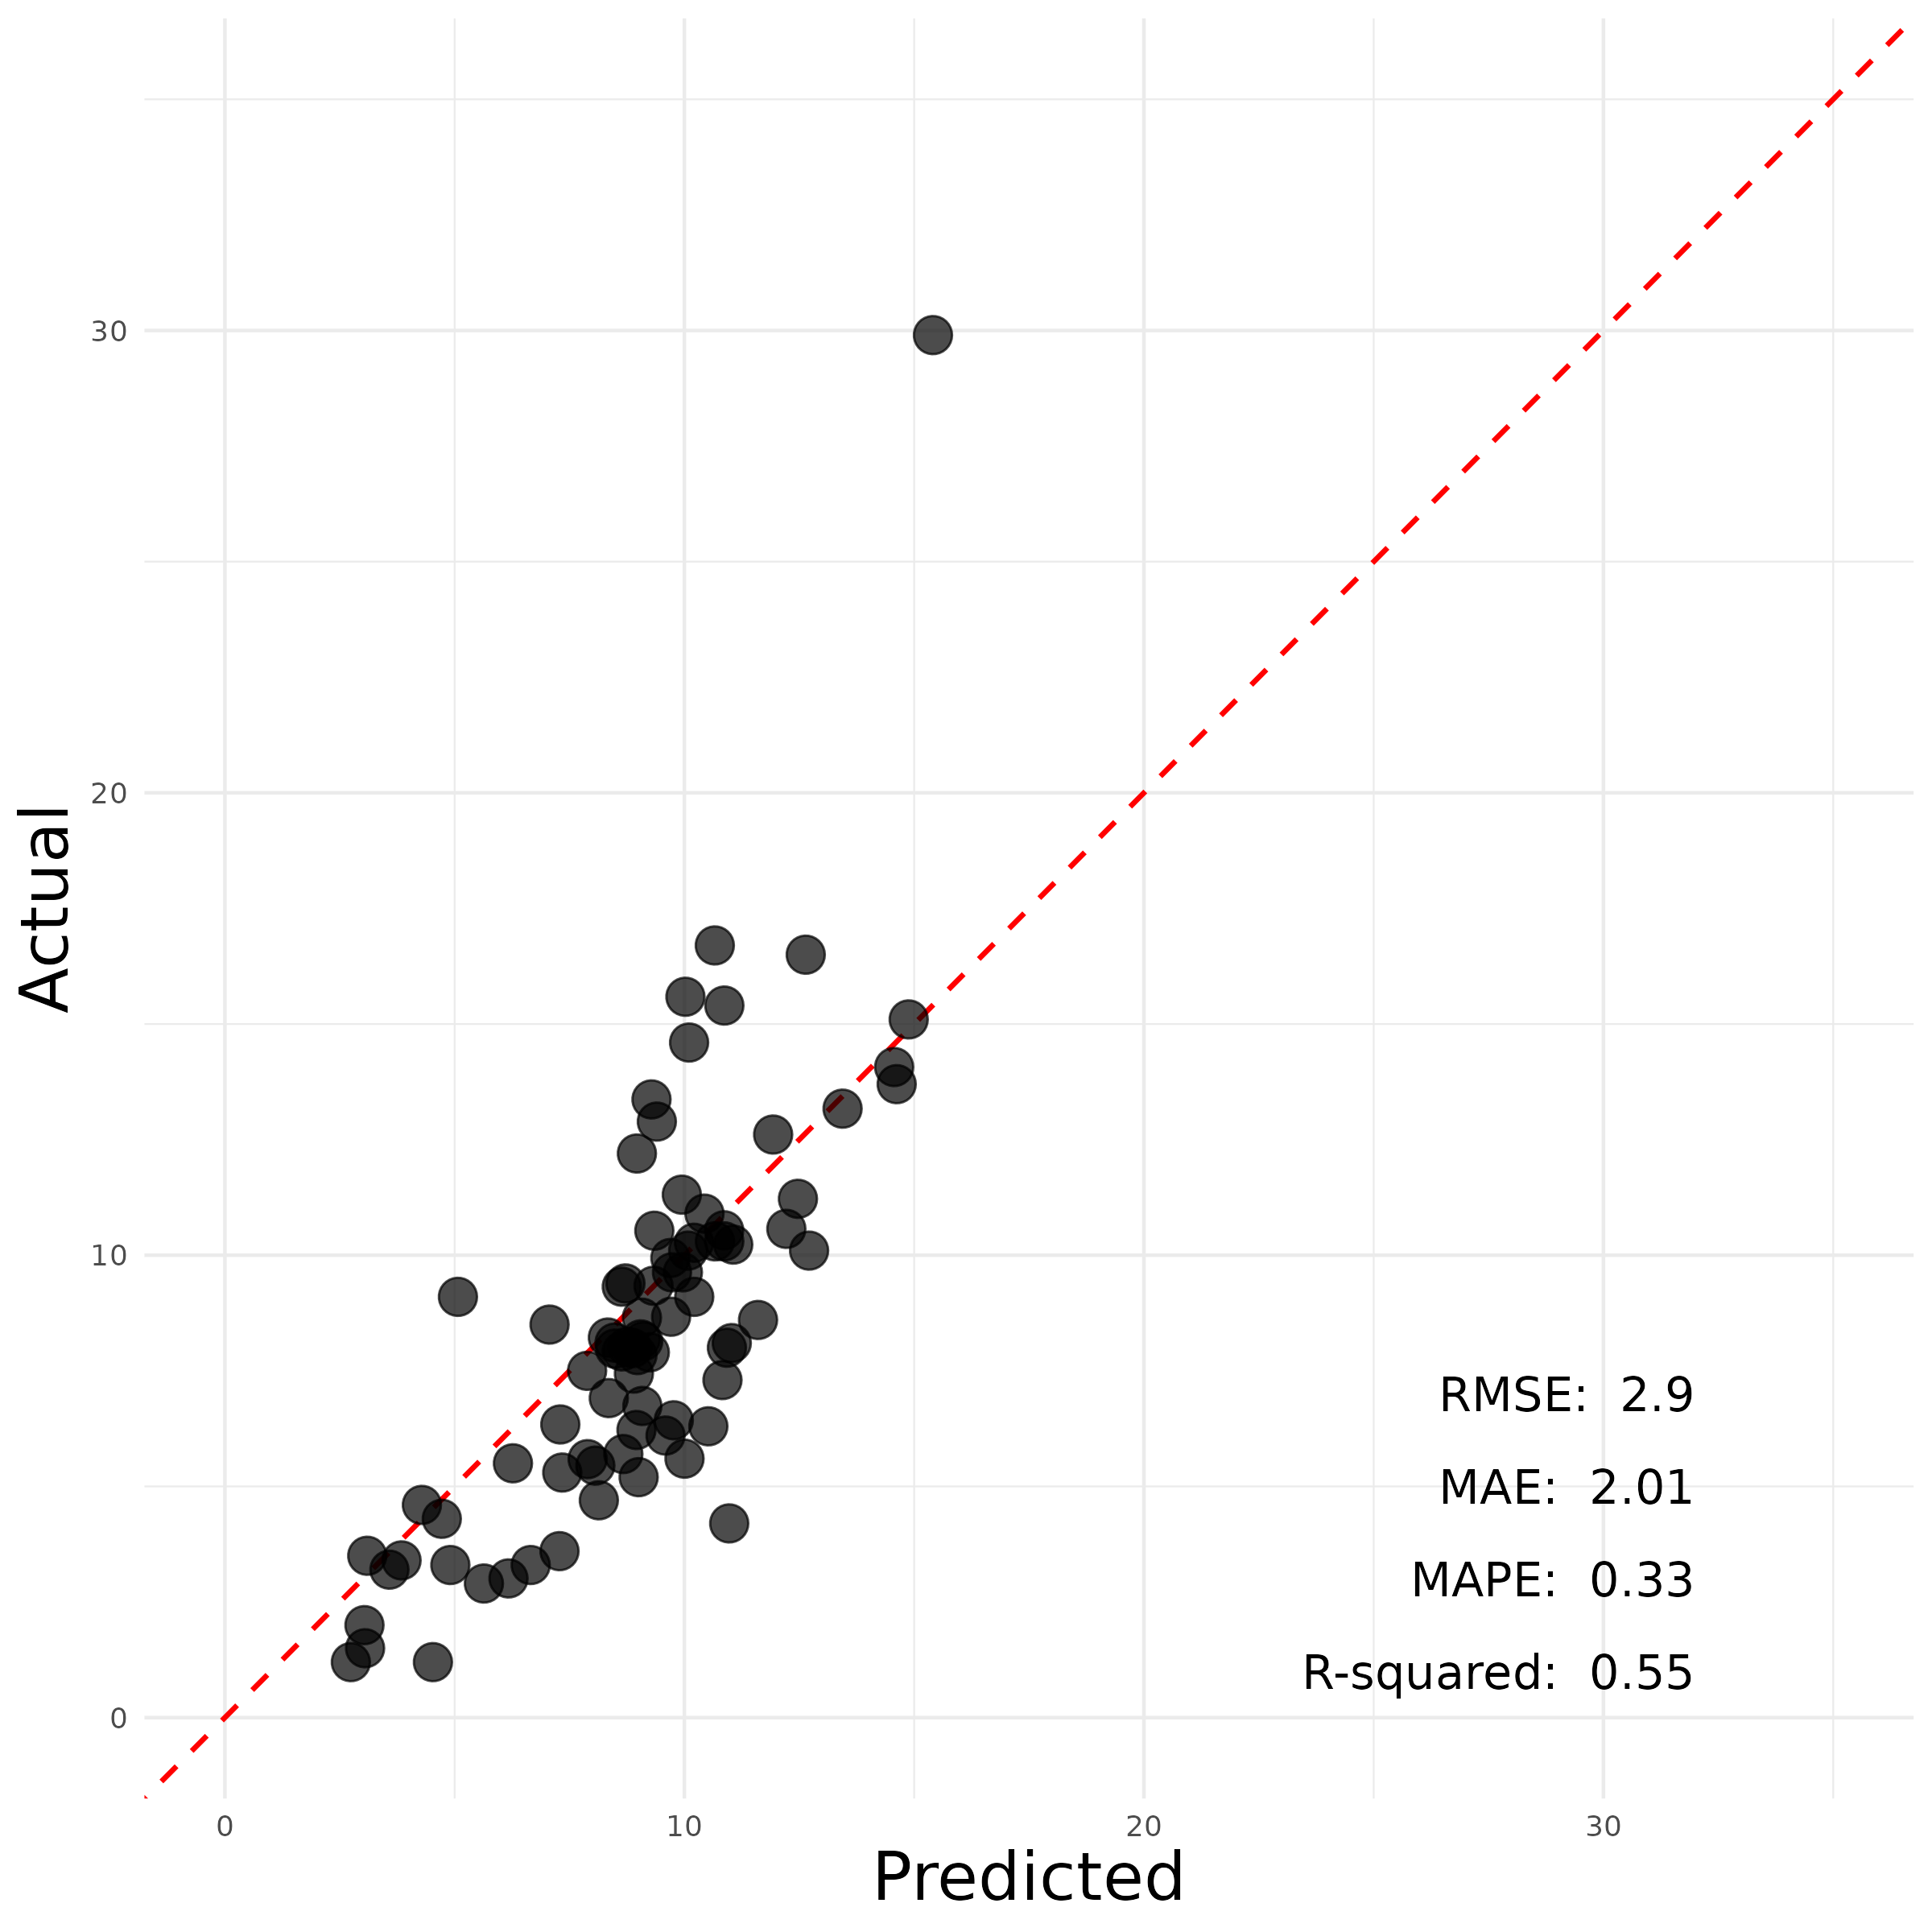
\includegraphics[width=0.3\linewidth,height=0.4\textheight]{Final_report_files/figure-latex/results_hree_test_best} 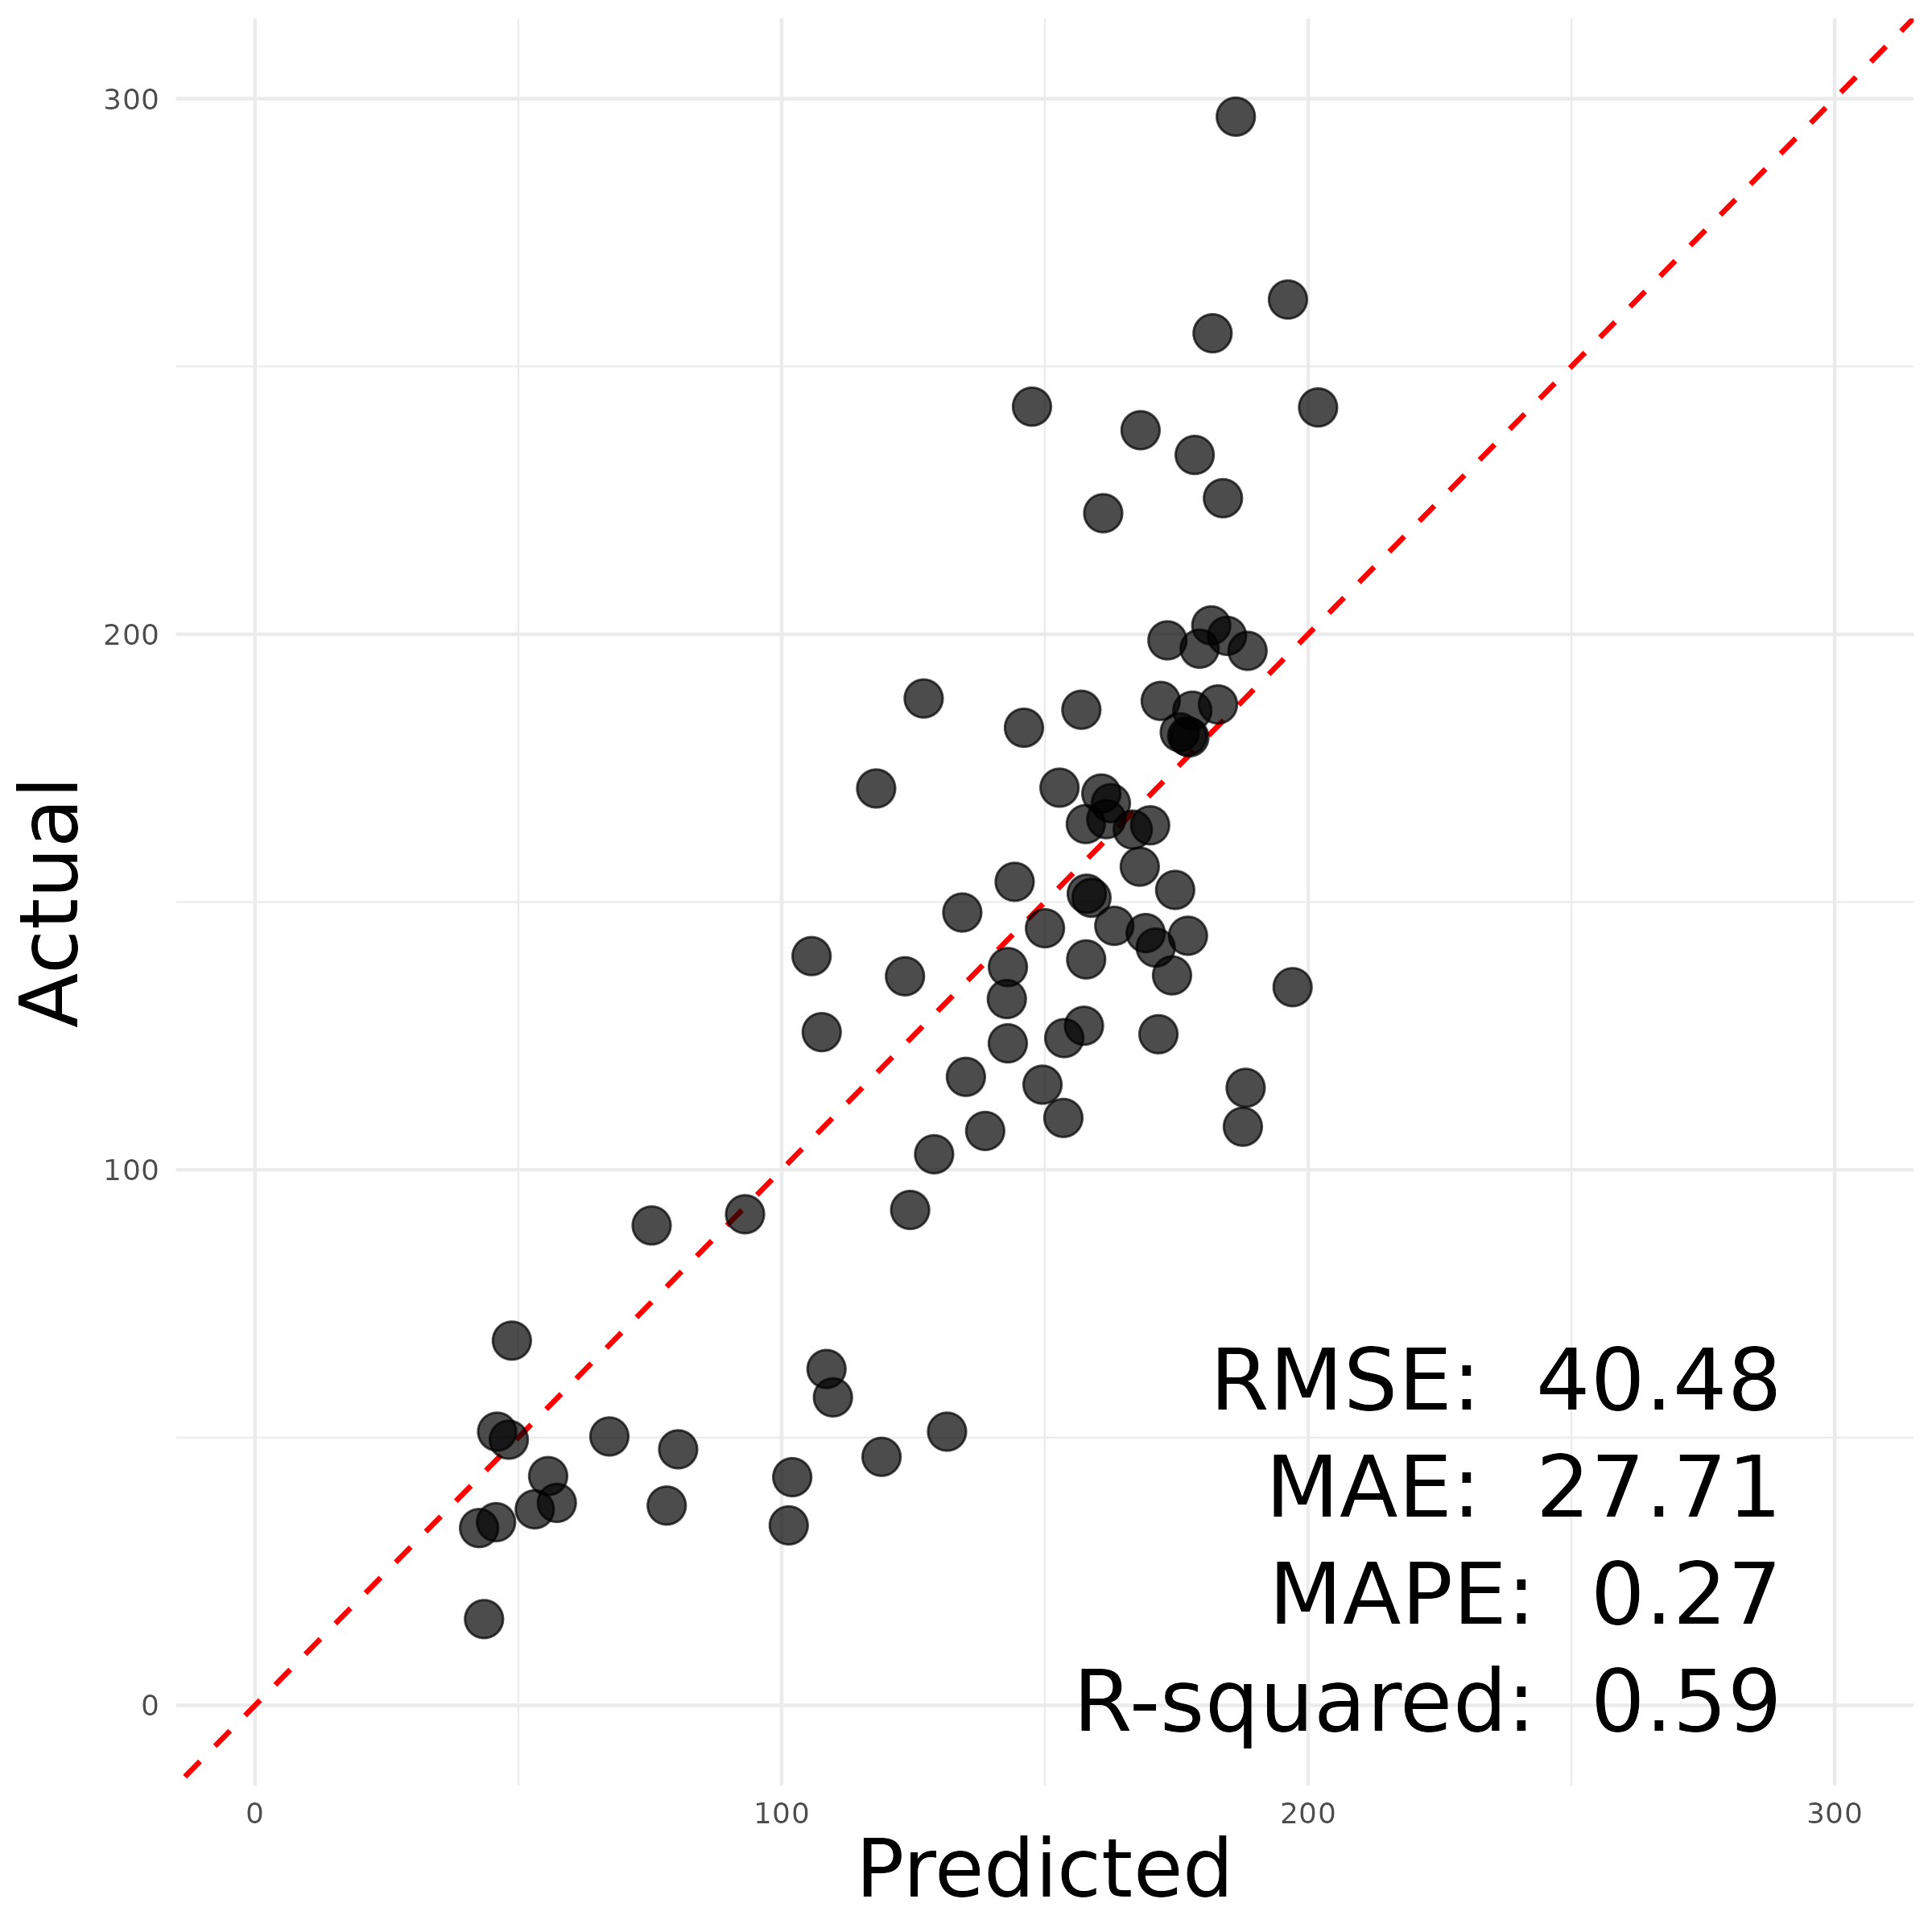
\includegraphics[width=0.3\linewidth,height=0.4\textheight]{Final_report_files/figure-latex/results_lree_test_best} 

}

\caption{Predicted vs Actual Values of the Best Models. From left to right: REE, HREE, LREE.}\label{fig:bestplot}
\end{figure}

The plot that compares predicted vs.~actual values of REE reveals moderate prediction performance by the model. With an RMSE of 47.57 and MAE of 33.85, the model demonstrates an average prediction error of roughly 47 units and an average absolute error of about 34 units, indicating that predictions are fairly close to the actual values but still have notable deviations. A MAPE of 26\% suggests that, on average, the model's predictions deviate by 26\% from the actual REE values, which is a slight improvement in accuracy compared to other similar models. The R-squared value of 0.62 indicates that 62\% of the variance in the actual values is captured by the model, showing a reasonable fit but still leaving significant room for error. In terms of key insights, the model performs relatively well for mid-range REE values, as the points are closely aligned along the diagonal line. However, the scatter becomes more pronounced at higher REE values (beyond 300), where the model underestimates the actual values, as observed by the upward spread of points above the line. This suggests that while the model captures general patterns, it faces challenges in predicting high REE values with precision, due to outliers and high range (max - min) value of REE as describe in Table \ref{tab:descstatsflt}.

From HREE plot, the model demonstrates reasonable predictive performance with some room for improvement. The RMSE of 3.33 indicates that, on average, the model's predictions deviate by about 3.33 units from the actual HREE values. The MAE of 2.13 suggests that the average absolute error is 2.13 units, indicating that the model tends to have relatively small errors overall. The MAPE of 29\% shows that the model's predictions are, on average, 29\% off from the actual values, which reflects moderate accuracy. The R-squared value of 0.46 reveals that 46\% of the variance in the actual HREE values is captured by the model, indicating that the model captures the general pattern but leaves a significant portion of variability unexplained. Some key insights from the plot, most data points cluster around lower values, particularly between 0 and 10 for both predicted and actual values, suggesting that the model predicts these ranges fairly well. However, for higher actual HREE values (above 10), the model tends to underestimate, as indicated by points above the diagonal line. Additionally, there is one outlier, particularly the one near 25 (of actual value), where the model considerably underpredicts. Overall, the model performs well for low to mid-range HREE values but struggles with higher values, leading to underestimation and some degree of error at the upper range.

Similar to other model where they have captured the general trend with some noticeable deviations, the same case observed from LREE plot. The RMSE of 38.44 and MAE of 29.6 indicate moderate errors in the predictions. MAE is slightly lower than RMSE, meaning that large errors (outliers) are not excessively frequent, but the general prediction error is still notable. A MAPE of 31\% highlights that the model's predictions are, on average, 31\% away from the actual values, indicating moderate accuracy. The R-squared value of 0.63 suggests that 63\% of the variance in the actual data is explained by the model, which shows a fair fit but leaves room for unexplained variance. Key insights from the plot include more accurate predictions in the lower to mid-range values of LREE, with a clustering of points near the diagonal line, while the model tends to underestimate higher actual LREE values, as shown by the increasing spread above 200. This underestimation at higher values signals some challenges in predicting extreme values accurately, which might be resulted from outliers and high range of LREE as describe in Table \ref{tab:descstatsflt}.

\subsection{Enrichment Analysis}\label{enrichment-analysis-1}

Figure \ref{fig:paaslvlcode} showcases the overall distribution of PAAS levels for all elements in the global project, which can give a holistic view of the enrichment and universality of each element's distribution. The cut-off threshold for element enrichment is represented by the red vertical dashed line, while the enriched and diminished samples are represented by green triangle and black circle, respectively.

Only a few elements, such as \texttt{Rhenium\ (Re)}, \texttt{Germanium\ (Ge)}, and \texttt{HREEs}, do not meet the detectable sample sizes due to either being absent or having a subtle presence, while the remaining elements are well-represented, with sufficient sample volumes observed in abundant concentrations.

Notably, elements like \texttt{Silver\ (Ag)} and \texttt{Gold\ (Au)} tend to show elevated enrichment in the majority of samples, with only one valid sample detected below the average. However, their spatial distribution is volatile. Even within the same region, completely opposite results can be observed, which poses challenges for mass production.

On the other hand, \texttt{Bismuth\ (Bi)} and \texttt{Lithium\ (Li)} present promising prospects for future growth. First and foremost, extraction from coal mines serves as a supplementary solution to ore reserves and is driven by market demand-supply dynamics. With the rising awareness of environmental sustainability and conservation, \texttt{Bi}, as a non-toxic alternative to \texttt{lead\ (Pb)}, has gained widespread attention,especially its alloy glasses for radiation protection purposes \autocite{Buriahi2021}. The global shifts towards EVs has also contributed to a surge in demand for lithium batteries. Additionally, compared with other elements with above-average levels, \texttt{Bi} and \texttt{Li} show higher levels of enrichment (more than 5 times the PAAS standard), with some specific projects detecting concentrations exceeding 10 times the PAAS standard.

Meanwhile, some instances of the element enrichment may be misleading due to the lab error. Despite a small number of valid samples, \texttt{Germanium\ (Ge)} stands out for its extremely enriched samples, displaying concentrations 30-40 times higher than the PAAS standard. Considering \texttt{Ge} is relatively rare in most natural environments and all these abnormal samples come from the same project (\texttt{Wandoan}), this seems more like a human error in statistical reporting from the laboratory. \texttt{Molybdenum\ (Mo)} and \texttt{Barium\ (Ba)} are also not typically enriched in coal seams. Their apparent enrichment might be incurred by the contamination of drilling fluids.

\begin{figure}
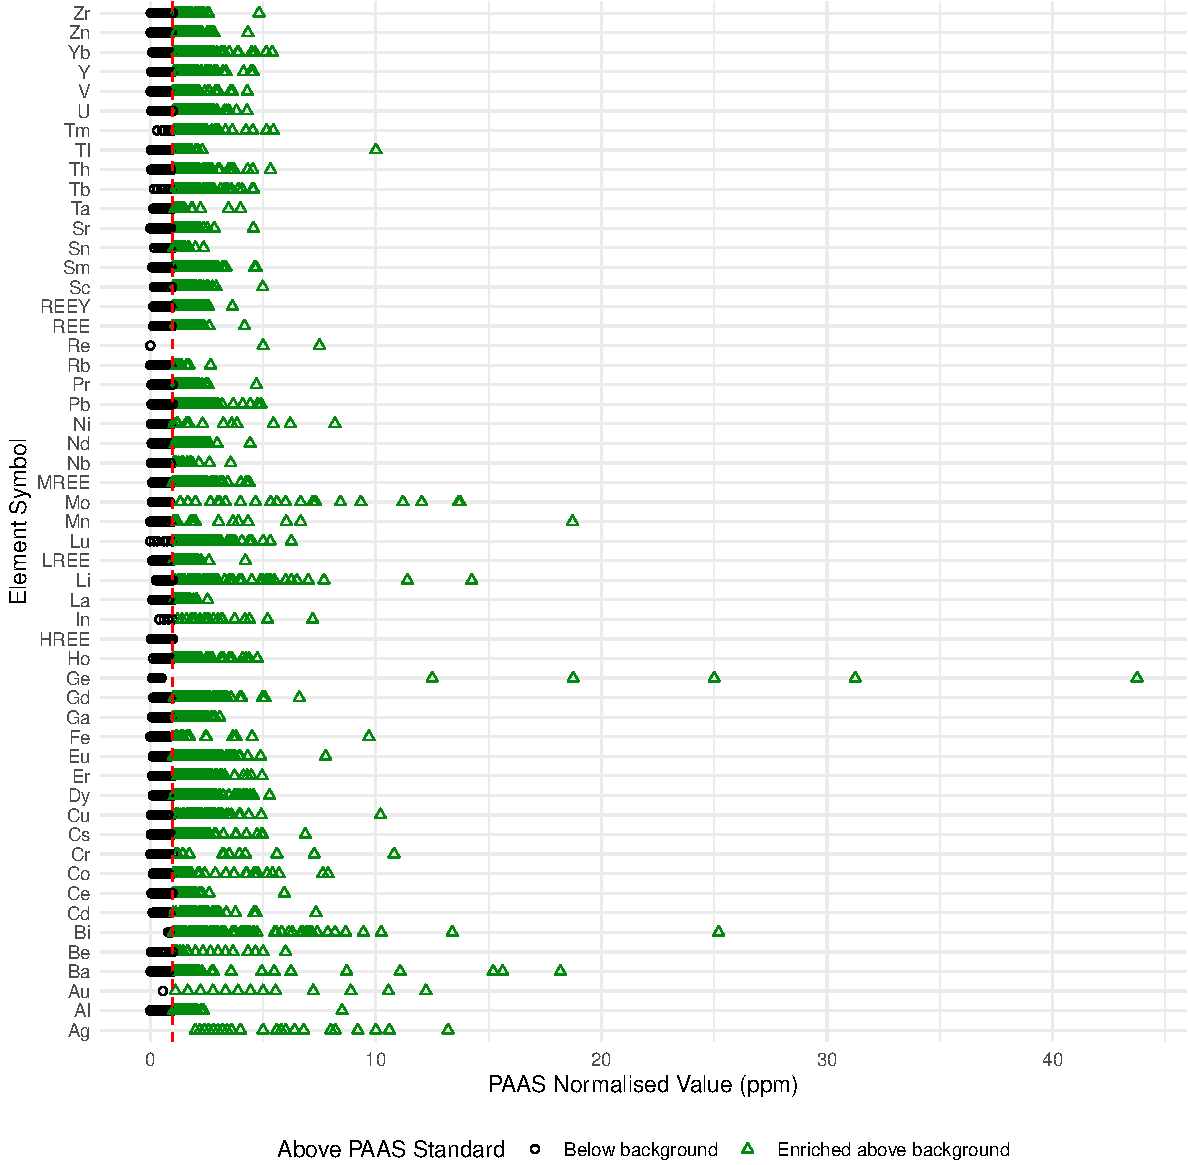
\includegraphics[width=1\linewidth,height=1\textheight]{Final_report_files/figure-latex/paaslvlcode-1} \caption{The distribution of element concentration with reference to PASS levels}\label{fig:paaslvlcode}
\end{figure}

Understanding the spatial variability and geochemical behavior across projects enables the subsequent exploration to focus on project regions with the highest potential yield. \hyperref[sec-appendixsix]{Appendix 6} provides a project breakdown of the distribution of element concentrations with reference to PASS levels. \texttt{Confidential\_A} and \texttt{Fort\ Cooper\ Coal\ Measure(FCCM)} are the primary potential enrichment areas. All measured elements exhibits a clear and widespread enrichment pattern, consistently maintaining an enrichment range of 1 to 5 times to the PAAS standard.

Moreover, \texttt{PowerPlant\ Ash} and \texttt{Confidential\_B} also show potential for development. Although their element enrichment is not as pronounced as in the two regions mentioned above, a significant number of samples still exhibit higher enrichment levels above the PAAS standard, particularly for critical elements such as \texttt{Aluminum\ (Al)} and \texttt{Titanium\ (Ti)} in \texttt{PowerPlant\ Ash}, LREEs and MREEs series in \texttt{Confidential\_B}. The variance among their samples is substantial, suggesting that the enrichment might be localised.

Finally, some impoverished projects are identified in the project breakdown, including \texttt{Unnamed}, \texttt{Coppabella}, \texttt{Newland} and \texttt{Metropolitian} among eight other projects. These projects show lower-than-average concentrations across the majority of measured elements, indicating limited economic potential under current conditions.

\section{Discussions}\label{discussions}

\subsection{Predictive Modelling}\label{predictive-modelling-3}

As all the best models have been thoroughly analysed, it is worth discussing whether these models can be considered `good models' for predicting REE, HREE, and LREE. Starting with the advantages, all the best models have RMSE and MAE values that are relatively close to the actual values, with some deviations. However, when these figures are compared to the standard deviation of each target variable, they fall significantly below the standard deviation. As shown in Table \ref{tab:descstatsflt}, the standard deviations of REE, HREE, and LREE are 78.9, 4.81, and 71, respectively. This indicates that the model's prediction errors are smaller than the natural variability in the target variables, meaning the models perform better than a simple mean-based prediction. \textcite{Moriasi2007} reported that if RMSE and MAE values are less than half of the standard deviation, the error can be considered low. In this case, the MAE values meet this criterion, while the RMSE values are slightly higher, which might be due to the model's higher sensitivity to outliers. Additionally, it is recommended to use the RMSE to Standard Deviation Ratio (RSR) to assess model performance, categorising models as `very good' if RSR is below 0.5, `good' if RSR is between 0.50 and 0.60, `satisfactory' if RSR is between 0.60 and 0.70, and `unsatisfactory' if RSR is above 0.70. The RSR of REEs and LREEs best models falls within the `good' category, however, HREEs best model categorised as `satisfactory' only. This suggest that all model are reasonably well if looking from RMSE stand point.

On the downside, the R-squared values of 0.62 (REE), 0.46 (HREE), and 0.63 (LREE) indicate that the models are only moderately strong in capturing the variability of the data. Ideally, an R-squared value above 0.8 would be desirable, but an R-squared above 0.5 is still acceptable \autocite{Moriasi2007}. Unfortunately, the HREE model is still below 0.5 level by a small margin. Furthermore, the MAPE values of 26\% (REE), 29\% (HREE), and 31\% (LREE) are relatively high, although they remain below the 50\% threshold.

There are several key considerations that justify classifying these models as good models. First, none of the elements from the ME-4ACD81 test show a high correlation with the target variables, making it challenging to produce highly accurate models. Second, a cost-benefit trade-off exists. Given that the ME-4ACD81 test is almost four times cheaper than the ME-MS81 test, these models are satisfactory, especially for businesses operating on tight budgets. Third, linked to the second point, the affordability of the ME-4ACD81 test allows for more samples to be tested, resulting in more data. With additional data, the model can be retrained, potentially improving its predictive accuracy. Therefore, it is reasonable to use samples tested via the ME-4ACD81 test. Finally, it should be noted that some errors were reported by the lab when inputting sample concentration values, leading to many outliers in the data. However, due to time constraints, the authors were unable to obtain corrected data.

\subsection{Enrichment Analysis}\label{enrichment-analysis-2}

With the escalating demand in the Australian market and the presence of enriched concentrations, Figure \ref{fig:paaslvlcode} suggests \texttt{Bi} and \texttt{Li} are the most promising elements for economic extraction. However, due to the different measurement protocols applied in element mapping across projects (e.g., ME-4ACD81 and ME-MS81 analyses), a significant amount of missing data for some elements is attributed to insufficient measurement precision and scope, rather than their absence in coal mines. Re-examining these project samples using a consistent testing method could help improve data integrity. Overall, the abnormal findings on enrichment align with recent studies from both local and international research, including \autocite{Sun2010} and \autocite{Hodgkinson2020}.

The project-wise breakdown serves as a valuable guideline for prospective extraction efforts by pinpointing areas of enrichment. A comprehensive and in-depth investigation is necessary to prioritise on \texttt{Confidential\_A} and \texttt{Fort\ Cooper\ Coal\ Measure\ (FCCM)}, where the distribution of enriched elements is both prevalent and consistently concentrated. To optimise resource input while maintaining high-quality output, a targeted study focusing on specific enriched elements may prove more effective in other potential area, such as \texttt{PowerPlant\ Ash} and \texttt{Confidential\_B}. Conversely, some projects that yielded underwhelming results should be excluded from future exploration efforts.

\section{Conclusion}\label{conclusion}

This study highlights the potential of using predictive modeling and enrichment analysis to evaluate the economic feasibility of extracting critical elements from coal mine waste in Australia. The predictive models, though exhibiting moderate R-squared values and relatively high MAPE, demonstrate reliable performance with RMSE and MAE values lower than the natural variability of the target variables. With additional calculation of RSR, it provides a fundamental reason to decide the models are falling under ``good'' and ``satisfactory'' category, thus making them valuable tools, especially when considering the cost-efficiency of the ME-4ACD81 lab analysis. The models are further justified by the trade-off between cost and prediction accuracy, as well as the potential for improvement with additional data. In terms of enrichment analysis, the discovery of economically feasible elements such as \texttt{Bi} and \texttt{Li}, along with areas like Fort Cooper and Confidential A, offers encouraging prospects for future extraction. While some areas provides promising further exploration, others with less potential can be deprioritised, enabling more efficient resource allocation.

This study encountered a key limitation that may have influenced the results: time constraints prevented authors from getting corrected lab data, which could have reduced outliers and improved model accuracy. Despite this, the findings remain valuable, though they should be interpreted with caution in light of this constraint. Furthermore, the study could benefit from additional data samples. Since the ME-4ACD81 test is more affordable, testing more samples is practical. With additional data, the model could be retrained to achieve a better prediction accuracy. Overall, this study provides a solid foundation for future research and practical applications in the economic extraction of critical elements from coal mine waste.

\newpage

\section{Appendix}\label{appendix}

\subsection{Appendix 1}\label{sec-appendixone}

\begingroup\fontsize{9}{11}\selectfont

\begin{longtabu} to \linewidth {>{\centering}X>{\centering}X>{\centering}X>{\centering}X>{\centering\arraybackslash}p{5cm}>{\centering}X}
\caption{\label{tab:celist}\textbf{Summary of Critical Elements: Production, Global Share, Projected Demand, and Usage}}\\
\toprule
Critical Element & Production (Kilotonnes) \textsuperscript{1} & Global Production (Percentage) & Projected Demand (Kilotonnes) \textsuperscript{2} & Usage \textsuperscript{3} & Level\\
\midrule
\endfirsthead
\caption[]{\label{tab:celist}\textbf{Summary of Critical Elements: Production, Global Share, Projected Demand, and Usage} \textit{(continued)}}\\
\toprule
Critical Element & Production (Kilotonnes) \textsuperscript{1} & Global Production (Percentage) & Projected Demand (Kilotonnes) \textsuperscript{2} & Usage \textsuperscript{3} & Level\\
\midrule
\endhead

\endfoot
\bottomrule
\multicolumn{6}{l}{\rule{0pt}{1em}\textsuperscript{a} Data collected in 2012.}\\
\multicolumn{6}{l}{\rule{0pt}{1em}\textsuperscript{b} 17 elements, including lanthanoid, Scandium (Sc), and Yttrium (Y).}\\
\multicolumn{6}{l}{\rule{0pt}{1em}\textsuperscript{c} 6 elements, including all transition metals in the d-block.}\\
\multicolumn{6}{l}{\rule{0pt}{1em}\textit{Source:} \textsuperscript{1} Skirrow et al., 2013 \& Coyne and Campbell, 2023; \textsuperscript{2} IEA, 2024b; \textsuperscript{3} Fortier et. al., 2018; Austrade, 2024}\\
\endlastfoot
Aluminum and derivative (Al) & 20 & 14 & - & Aerospace alloys, Coating in Li-ion batteries & \cellcolor[HTML]{F7D7DC}{High}\\
Cobalt (Co) & 5.9 & 3 & 243.03 & Li-ion battery cathodes, stainless steels, superalloys & \cellcolor[HTML]{F7D7DC}{High}\\
Gallium (Ga) & - & - & 0.25 & Radar, light-emitting diodes (LEDs), photovoltaics films & \cellcolor[HTML]{F7D7DC}{High}\\
Germanium (Ge) & - & - & 0.03 & Fiber/infrared optics, Polymerization Catalysts, 
          semiconductors & \cellcolor[HTML]{F7D7DC}{High}\\
Lithium(Li) & 61 & 47 & 615.55 & Li-ion batteries, aerospace alloys, ceramics & \cellcolor[HTML]{F7D7DC}{High}\\
\addlinespace
Magnesium(Mg) & 2.6 & 10 & 30.95 & Pyrotechnics, nanocomposites in automotive/aerospace & \cellcolor[HTML]{F7D7DC}{High}\\
Manganese(Mn) & 3.3 & 17 & 855 & Steel, Agricultural fertilizer, lightweight alloys & \cellcolor[HTML]{F7D7DC}{High}\\
Nickel(Ni) & 150\textsuperscript{a} & 4.5 & 2792.68 & Cathodes of Li-ion batteries, Non-ferrous alloys & \cellcolor[HTML]{F7D7DC}{High}\\
Rare-earth elements (REE)\textsuperscript{b} & 18 & 6 & 61.96 & Catalysts, magnets, guidance, lasers & \cellcolor[HTML]{F7D7DC}{High}\\
Silicon (Si) & 0.05 & 1 & 2025 & Solar PVs, Silicon wafers in electronic and photovoltaic cells & \cellcolor[HTML]{F7D7DC}{High}\\
\addlinespace
Tantalum (Ta) & 0.057 & 3 & 0.44 & Micro-capacitors, superalloys & \cellcolor[HTML]{F7D7DC}{High}\\
Titanium (Ti) & 0.85 & 8.4 & 22.69 & Aerospace and marine alloys, pigment & \cellcolor[HTML]{F7D7DC}{High}\\
Tungsten (W) & - & - & 0.17 & Lightning, Cutting and drilling tools, 
          catalysts & \cellcolor[HTML]{F7D7DC}{High}\\
Vanadium (V) & - & - & 35.23 & Steel or aerospace alloys & \cellcolor[HTML]{F7D7DC}{High}\\
Zirconium (Zr) & 0.5 & 36 & 11.14 & Cladding fuel rods, nuclear reactors & \cellcolor[HTML]{F7D7DC}{High}\\
\addlinespace
Antimony (Sb) & 4 & 4 & - & Flame retardant, lead-acid batteries & \cellcolor[HTML]{FDA}{Moderate}\\
Arsenic (As) & - & - & 0.55 & Microwave communications, pesticides, semiconductors & \cellcolor[HTML]{FDA}{Moderate}\\
Beryllium (Be) & - & - & - & Satellite communications, lightweight alloys & \cellcolor[HTML]{FDA}{Moderate}\\
Bismuth (Bi) & - & - & - & Pharmaceuticals, lead-free solders, cosmetics & \cellcolor[HTML]{FDA}{Moderate}\\
Chromium (Cr) & 66.1 & 0.3 & 823.7 & Steel or aerospace alloys, leather tanning & \cellcolor[HTML]{FDA}{Moderate}\\
\addlinespace
Fluorine (F) & - & - & - & Refrigerants, dental care, 
          nuclear processing & \cellcolor[HTML]{FDA}{Moderate}\\
Graphite (Gr) & - & - & 8406.7 & Rechargeable batteries, semiconductors and sensors, water filtration & \cellcolor[HTML]{FDA}{Moderate}\\
Hafnium (Hf) & - & - & 0.02 & Nuclear reactors, 
          aerospace alloys & \cellcolor[HTML]{FDA}{Moderate}\\
Indium (In) & - & - & 0.17 & Flat-panel displays, low-Melting Alloys, semiconductors & \cellcolor[HTML]{FDA}{Moderate}\\
Molybdenum (Mo) & - & - & 104.44 & Improving strength and corrosion resistance 
          in steel alloys & \cellcolor[HTML]{FDA}{Moderate}\\
\addlinespace
Niobium (Nb) & - & - & 1.97 & High-Strength Low-Alloy (HSLA) Steel, superalloys, superconductors, welding & \cellcolor[HTML]{FDA}{Moderate}\\
Platinum-group elements (PGE)\textsuperscript{c} & <0.01 & <0.01 & 0.03 & Catalysts, jewelry, thermocouples & \cellcolor[HTML]{FDA}{Moderate}\\
Rhenium (Re) & - & - & - & Superalloys, catalysts, electrical Contacts, filaments & \cellcolor[HTML]{FDA}{Moderate}\\
Selenium(Se) & - & - & 0.26 & Alloying agents, solar cells, 
          glass production & \cellcolor[HTML]{FDA}{Moderate}\\
Tellurium (Te) & - & - & 1.55 & Copper or steel alloys, semiconductors, solar cells, thermoelectric Materials & \cellcolor[HTML]{FDA}{Moderate}\\*
\end{longtabu}
\endgroup{}

\newpage

\subsection{Appendix 2}\label{sec-appendixtwo}

\begingroup\fontsize{9}{11}\selectfont

\begin{longtabu} to \linewidth {>{\centering}X>{\centering}X>{\centering}X>{\centering}X>{\centering}X}
\caption{\label{tab:concentration}\textbf{Summary of Hodginkson's research on critical element mapping in coal mines}}\\
\toprule
Critical Element & PAAS Standard & Average Concentration (ppm) & Highest Concentration (ppm) & Above Crustal Average (Percentage)\\
\midrule
\endfirsthead
\caption[]{\label{tab:concentration}\textbf{Summary of Hodginkson's research on critical element mapping in coal mines} \textit{(continued)}}\\
\toprule
Critical Element & PAAS Standard & Average Concentration (ppm) & Highest Concentration (ppm) & Above Crustal Average (Percentage)\\
\midrule
\endhead

\endfoot
\bottomrule
\multicolumn{5}{l}{\rule{0pt}{1em}\textit{Source: } Adapted from Hodginkson et al., 2020}\\
\endlastfoot
\addlinespace[0.3em]
\multicolumn{5}{l}{\textbf{Coal Seam \& Associate}}\\
\hspace{1em}Lithium & 21.0 & 13.7 & \textbf{25} & 22\\
\hspace{1em}REE & 184.0 & 115.8 & \textbf{205} & 11\\
\hspace{1em}Cobalt & 17.0 & 16.9 & \textbf{30} & 44\\
\hspace{1em}Nickel & 47.0 & 11.2 & 40 & 0\\
\hspace{1em}Tantalum & 1.0 & 0.33 & 1 & 33\\
\hspace{1em}Vanadium & 97.0 & 85.6 & \textbf{140} & 22\\
\hspace{1em}Zirconium & 193.0 & 102.1 & 160 & 0\\
\hspace{1em}Gallium & 17.0 & 12.3 & \textbf{25} & 44\\
\hspace{1em}Bismuth & 0.2 & \textbf{0.59} & \textbf{1} & 67\\
\hspace{1em}Chromium & 92.0 & 14.33 & 51 & 0\\
\hspace{1em}Niobium & 12.0 & 7.9 & \textbf{32} & 11\\
\hspace{1em}Molybdenum & 1.0 & \textbf{1.33} & \textbf{3} & 78\\
\addlinespace[0.3em]
\multicolumn{5}{l}{\textbf{Siltstone \& Mudstone}}\\
\hspace{1em}Lithium & 21.0 & 17.2 & \textbf{28} & 33\\
\hspace{1em}REE & 184.0 & 138.8 & \textbf{189} & 17\\
\hspace{1em}Cobalt & 17.0 & \textbf{39.3} & \textbf{134} & 67\\
\hspace{1em}Nickel & 47.0 & 25.8 & \textbf{73} & 33\\
\hspace{1em}Tantalum & 1.0 & 0.2 & 1 & 17\\
\hspace{1em}Vanadium & 97.0 & \textbf{102} & \textbf{225} & 33\\
\hspace{1em}Zirconium & 193.0 & 116.8 & \textbf{243} & 17\\
\hspace{1em}Gallium & 17.0 & 15 & \textbf{22} & 33\\
\hspace{1em}Bismuth & 0.2 & 0.18 & \textbf{0.4} & 67\\
\hspace{1em}Chromium & 92.0 & 51.33 & \textbf{266} & 17\\
\hspace{1em}Niobium & 12.0 & 4.67 & 8 & 0\\
\hspace{1em}Molybdenum & 1.0 & 0.67 & 1 & 67\\
\addlinespace[0.3em]
\multicolumn{5}{l}{\textbf{Tuffaceous Rocks}}\\
\hspace{1em}Lithium & 21.0 & \textbf{21.5} & \textbf{105} & 12\\
\hspace{1em}REE & 184.0 & \textbf{244} & \textbf{441} & 88\\
\hspace{1em}Cobalt & 17.0 & 9.25 & \textbf{19} & 12\\
\hspace{1em}Nickel & 47.0 & 3.75 & 30 & 0\\
\hspace{1em}Tantalum & 1.0 & \textbf{1.1} & \textbf{2} & 100\\
\hspace{1em}Vanadium & 97.0 & 27.9 & 70 & 0\\
\hspace{1em}Zirconium & 193.0 & 153.75 & \textbf{282} & 25\\
\hspace{1em}Gallium & 17.0 & \textbf{32.25} & \textbf{37} & 100\\
\hspace{1em}Bismuth & 0.2 & \textbf{0.71} & \textbf{1.2} & 100\\
\hspace{1em}Chromium & 92.0 & 0 & 0 & 0\\
\hspace{1em}Niobium & 12.0 & 9.63 & \textbf{18} & 25\\
\hspace{1em}Molybdenum & 1.0 & 1 & \textbf{5} & 50\\*
\end{longtabu}
\endgroup{}

\subsection{Appendix 3}\label{sec-appendixthree}

\begingroup\fontsize{10}{12}\selectfont

\begin{longtabu} to \linewidth {>{\centering}X>{\centering}X}
\caption{\label{tab:cutoff-grade}\textbf{Selected critical elements with their suggested cut-off grade (ppm)}}\\
\toprule
Critical Element & Suggested Cut-off Grade\\
\midrule
\endfirsthead
\caption[]{\label{tab:cutoff-grade}\textbf{Selected critical elements with their suggested cut-off grade (ppm)} \textit{(continued)}}\\
\toprule
Critical Element & Suggested Cut-off Grade\\
\midrule
\endhead

\endfoot
\bottomrule
\multicolumn{2}{l}{\rule{0pt}{1em}\textit{Source: } Adapted from Dai and Finkelman, 2018}\\
\endlastfoot
U & 1000\\
Ge & 300\\
V & 1000\\
Se & 500–800\\
Ga & 100 (50)\\
REE & 1000\\
Y & 300\\
Sc & 100\\
Nb & 300\\
Zr & 2000\\
Mo & 1000\\
Re & 1\\
Wi & 1000\\
Au + Pt + Pd & 2\\
Ag & 10\\
Be & 300\\
Sb & 1000\\
Cs & 150\\*
\end{longtabu}
\endgroup{}

\newpage

\subsection{Appendix 4}\label{sec-appendixfour}

\begingroup\fontsize{9}{11}\selectfont

\begin{longtabu} to \linewidth {>{\centering}X>{}c>{\centering}X>{\centering}X>{\centering}X>{\centering}X>{\centering}X}
\caption{\label{tab:descstats}\textbf{Descriptive Statistics of Elements' Normalised Value}}\\
\toprule
Element Symbol & min & max & mean & median & sd & kurtosis\\
\midrule
\endfirsthead
\caption[]{\label{tab:descstats}\textbf{Descriptive Statistics of Elements' Normalised Value} \textit{(continued)}}\\
\toprule
Element Symbol & min & max & mean & median & sd & kurtosis\\
\midrule
\endhead

\endfoot
\bottomrule
\endlastfoot
Ag & 2.00 & 13.20 & 4.14 & 3.60 & 2.39 & 5.78\\
Al & 0.00 & 8.50 & 0.84 & 0.44 & 0.98 & 34.19\\
Au & 0.56 & 12.22 & 3.52 & 3.33 & 2.06 & 7.76\\
Ba & 0.01 & 18.18 & 1.11 & 0.75 & 2.03 & 43.45\\
Be & 0.03 & 6.00 & 1.13 & 0.67 & 1.13 & 7.16\\
\addlinespace
Bi & 0.79 & 25.20 & 3.69 & 2.40 & 3.30 & 17.82\\
Cd & 0.10 & 7.35 & 1.27 & 0.92 & 1.11 & 9.84\\
Ce & 0.06 & 5.94 & 0.96 & 0.99 & 0.59 & 21.06\\
Co & 0.12 & 7.88 & 0.91 & 0.59 & 1.13 & 17.66\\
Cr & 0.01 & 10.81 & 0.44 & 0.20 & 1.05 & 54.64\\
\addlinespace
Cs & 0.02 & 6.87 & 1.07 & 0.92 & 0.91 & 12.86\\
Cu & 0.04 & 10.20 & 1.68 & 1.88 & 1.16 & 13.14\\
Dy & 0.11 & 5.29 & 1.52 & 1.52 & 0.85 & 5.57\\
Er & 0.09 & 4.96 & 1.40 & 1.32 & 0.82 & 6.38\\
Eu & 0.11 & 7.77 & 1.68 & 1.65 & 0.97 & 8.54\\
\addlinespace
Fe & 0.00 & 9.69 & 0.47 & 0.18 & 1.07 & 45.05\\
Ga & 0.08 & 3.08 & 1.29 & 1.29 & 0.68 & 2.15\\
Gd & 0.13 & 6.61 & 1.59 & 1.51 & 0.90 & 7.42\\
Ge & 0.09 & 43.75 & 7.48 & 0.34 & 13.03 & 3.65\\
HREE & 0.04 & 1.00 & 0.28 & 0.27 & 0.16 & 6.71\\
\addlinespace
Ho & 0.12 & 4.75 & 1.35 & 1.31 & 0.77 & 5.96\\
In & 0.40 & 7.20 & 1.43 & 1.00 & 1.12 & 9.58\\
LREE & 0.09 & 4.21 & 1.02 & 1.06 & 0.54 & 6.99\\
La & 0.10 & 2.54 & 0.87 & 0.93 & 0.48 & 2.57\\
Li & 0.25 & 14.25 & 2.39 & 2.00 & 1.97 & 9.53\\
\addlinespace
Lu & 0.00 & 6.25 & 1.54 & 1.44 & 0.92 & 7.07\\
MREE & 0.09 & 4.38 & 1.36 & 1.34 & 0.76 & 5.95\\
Mn & 0.00 & 18.72 & 0.59 & 0.11 & 1.88 & 66.53\\
Mo & 0.07 & 13.73 & 2.97 & 2.67 & 2.19 & 10.24\\
Nb & 0.04 & 3.57 & 0.62 & 0.65 & 0.40 & 16.60\\
\addlinespace
Nd & 0.07 & 4.42 & 1.15 & 1.22 & 0.64 & 4.69\\
Ni & 0.02 & 8.18 & 0.39 & 0.16 & 0.87 & 44.10\\
Pb & 0.05 & 4.91 & 1.28 & 1.24 & 0.86 & 6.14\\
Pr & 0.06 & 4.70 & 1.03 & 1.09 & 0.60 & 7.45\\
REE & 0.13 & 4.17 & 1.09 & 1.13 & 0.54 & 6.57\\
\addlinespace
REEY & 0.14 & 3.64 & 1.12 & 1.15 & 0.53 & 4.60\\
Rb & 0.00 & 2.67 & 0.47 & 0.44 & 0.40 & 5.92\\
Re & 0.00 & 7.50 & 4.29 & 5.00 & 3.13 & 1.79\\
Sc & 0.16 & 4.99 & 1.14 & 1.19 & 0.61 & 8.48\\
Sm & 0.09 & 4.69 & 1.42 & 1.46 & 0.78 & 4.17\\
\addlinespace
Sn & 0.18 & 2.36 & 0.73 & 0.65 & 0.35 & 6.86\\
Sr & 0.01 & 4.57 & 0.95 & 0.92 & 0.61 & 6.97\\
Ta & 0.13 & 4.00 & 0.87 & 0.92 & 0.48 & 14.45\\
Tb & 0.16 & 4.58 & 1.38 & 1.36 & 0.76 & 5.58\\
Th & 0.04 & 5.33 & 1.17 & 1.11 & 0.85 & 6.38\\
\addlinespace
Tl & 0.03 & 10.00 & 1.94 & 0.72 & 3.12 & 5.78\\
Tm & 0.30 & 5.45 & 1.45 & 1.36 & 0.82 & 7.68\\
U & 0.05 & 4.29 & 1.29 & 1.30 & 0.81 & 3.22\\
V & 0.02 & 4.30 & 1.04 & 1.10 & 0.67 & 5.96\\
Y & 0.05 & 4.57 & 1.28 & 1.25 & 0.76 & 6.44\\
\addlinespace
Yb & 0.09 & 5.41 & 1.46 & 1.40 & 0.85 & 6.36\\
Zn & 0.01 & 4.32 & 0.92 & 0.93 & 0.70 & 4.13\\
Zr & 0.02 & 4.82 & 0.92 & 0.98 & 0.59 & 9.67\\*
\end{longtabu}
\endgroup{}

\newpage

\subsection{Appendix 5}\label{sec-appendixfive}

\begin{figure}

{\centering 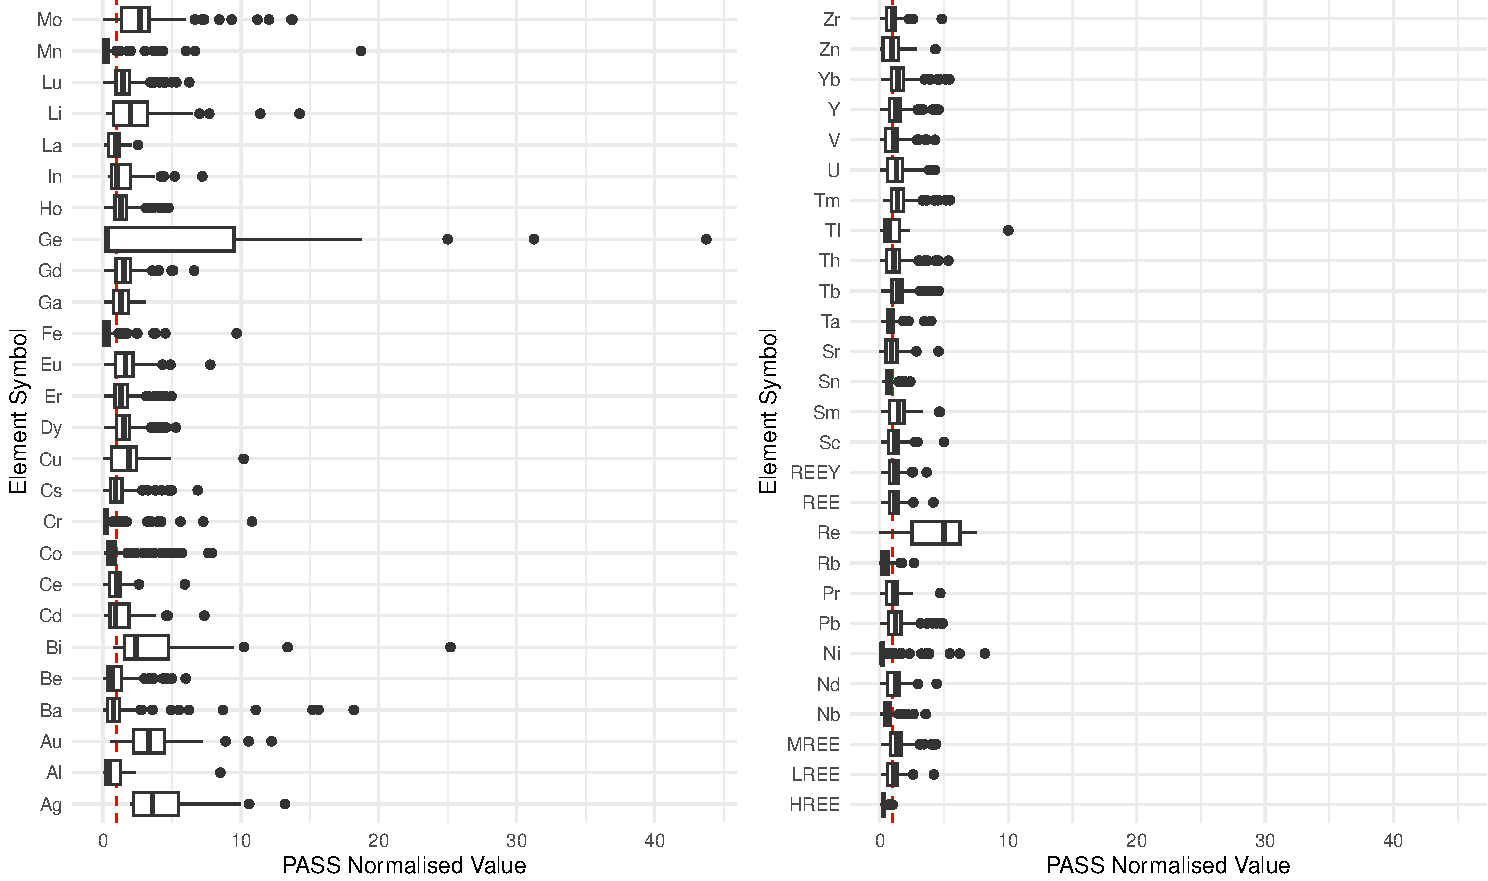
\includegraphics[width=1\linewidth]{Final_report_files/figure-latex/element-dist-1} 

}

\caption{Distribution of Critical Elements (Box-Plot)}\label{fig:element-dist}
\end{figure}

\newpage

\subsection{Appendix 6}\label{sec-appendixsix}

\begin{figure}
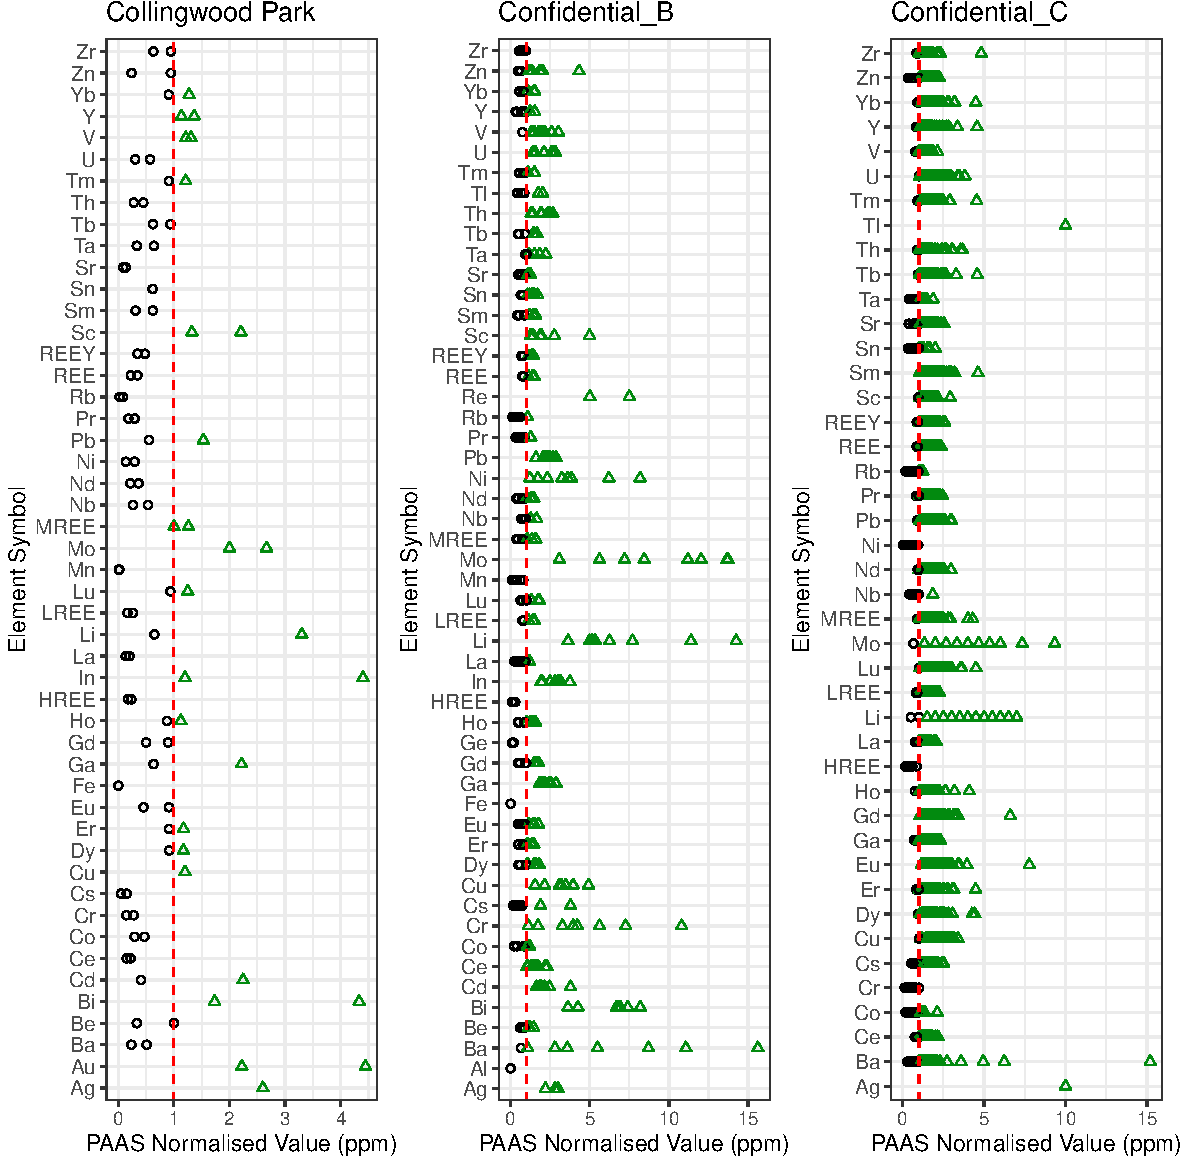
\includegraphics[width=1\linewidth,height=1\textheight]{Final_report_files/figure-latex/regionalbk1-1} \caption{Project breakdown for the distribution of element concentration with reference to PASS levels}\label{fig:regionalbk1}
\end{figure}

\newpage

\begin{figure}
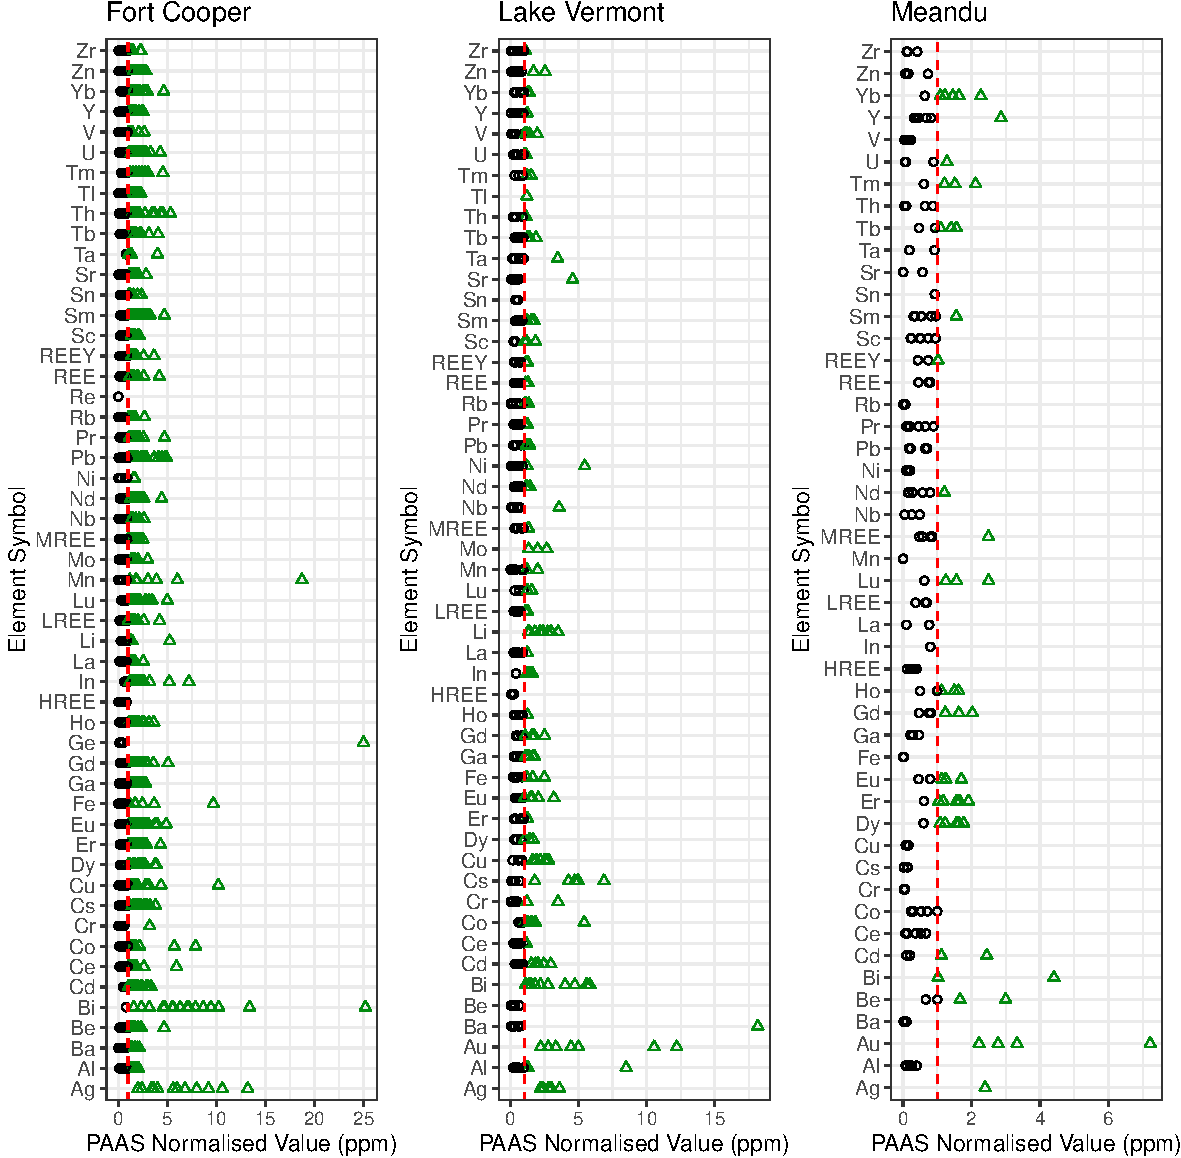
\includegraphics[width=1\linewidth,height=1\textheight]{Final_report_files/figure-latex/regionalbk2-1} \caption{Project breakdown for the distribution of element concentration with reference to PASS levels}\label{fig:regionalbk2}
\end{figure}

\newpage

\begin{figure}
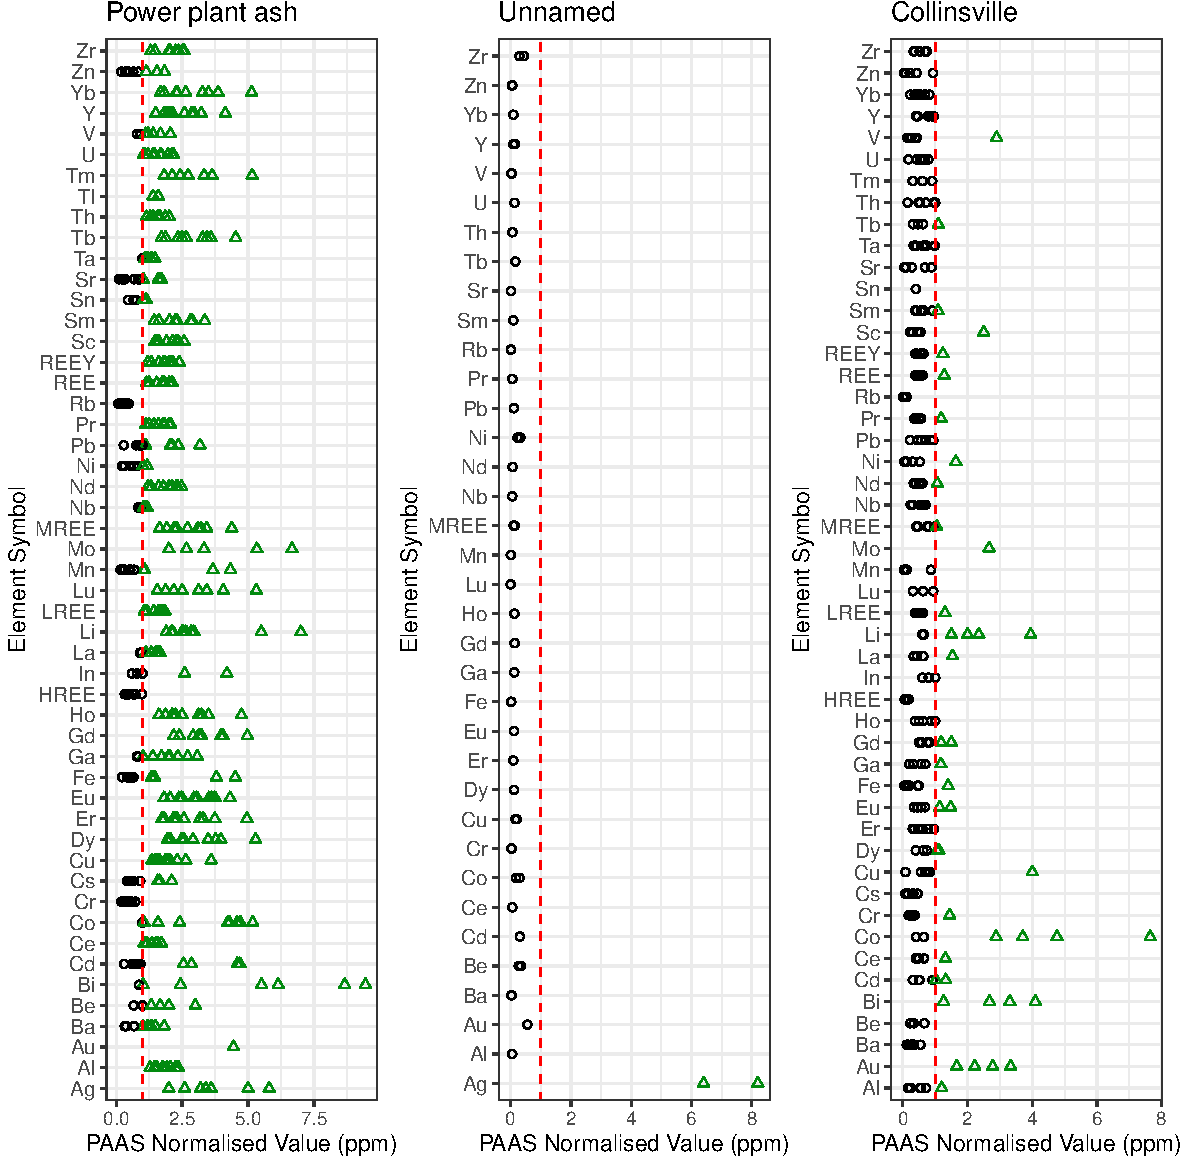
\includegraphics[width=1\linewidth,height=1\textheight]{Final_report_files/figure-latex/regionalbk3-1} \caption{Project breakdown for the distribution of element concentration with reference to PASS levels}\label{fig:regionalbk3}
\end{figure}

\newpage

\begin{figure}
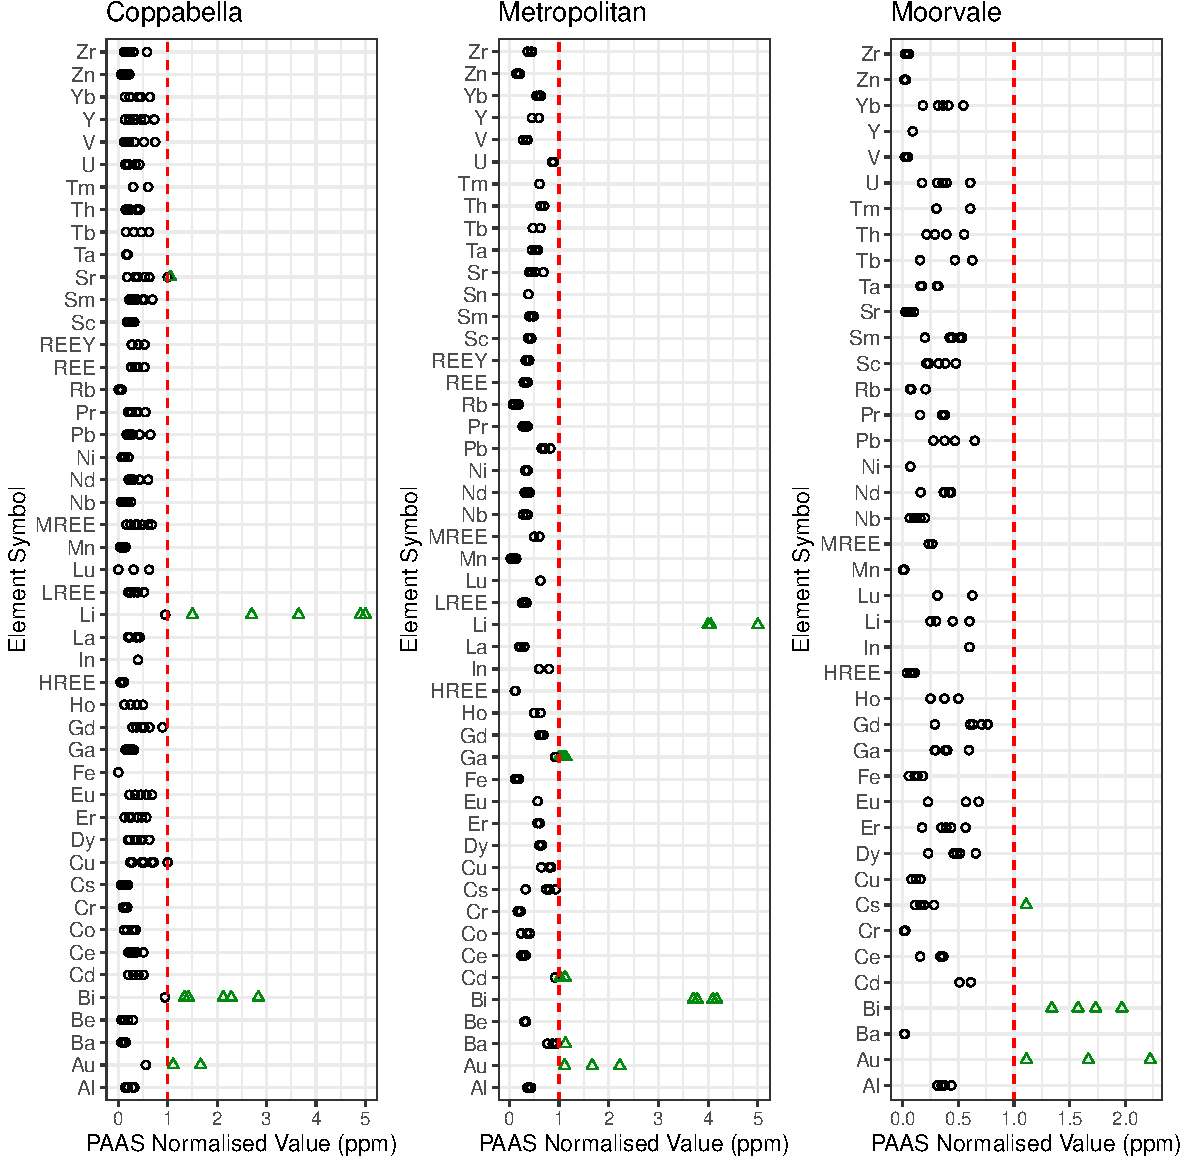
\includegraphics[width=1\linewidth,height=1\textheight]{Final_report_files/figure-latex/regionalbk4-1} \caption{Project breakdown for the distribution of element concentration with reference to PASS levels}\label{fig:regionalbk4}
\end{figure}

\newpage

\begin{figure}
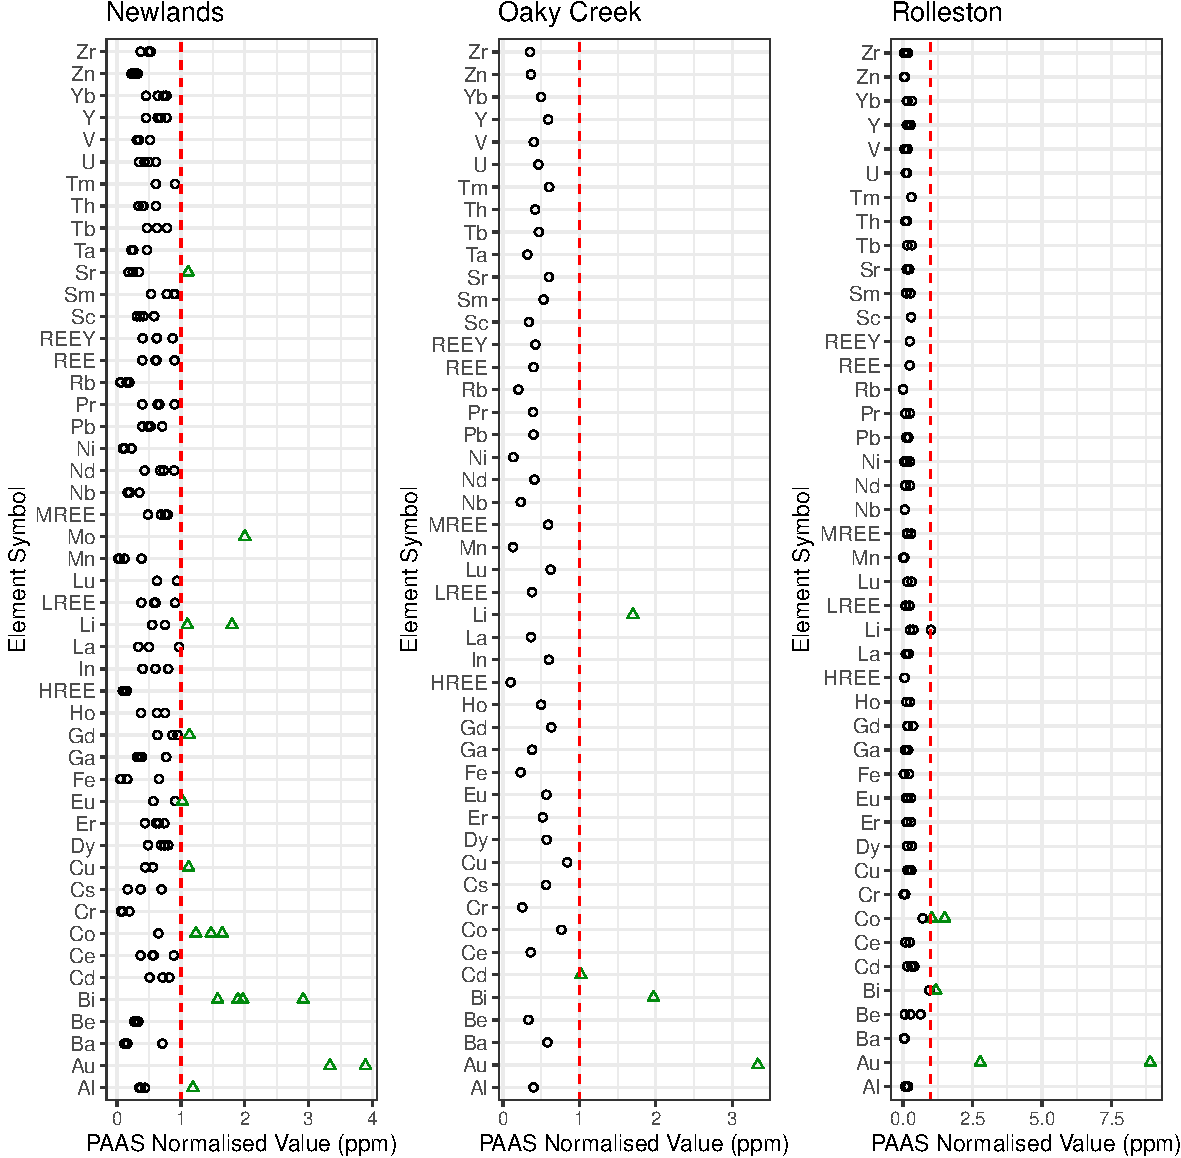
\includegraphics[width=1\linewidth,height=1\textheight]{Final_report_files/figure-latex/regionalbk5-1} \caption{Project breakdown for the distribution of element concentration with reference to PASS levels}\label{fig:regionalbk5}
\end{figure}

\newpage

\begin{figure}
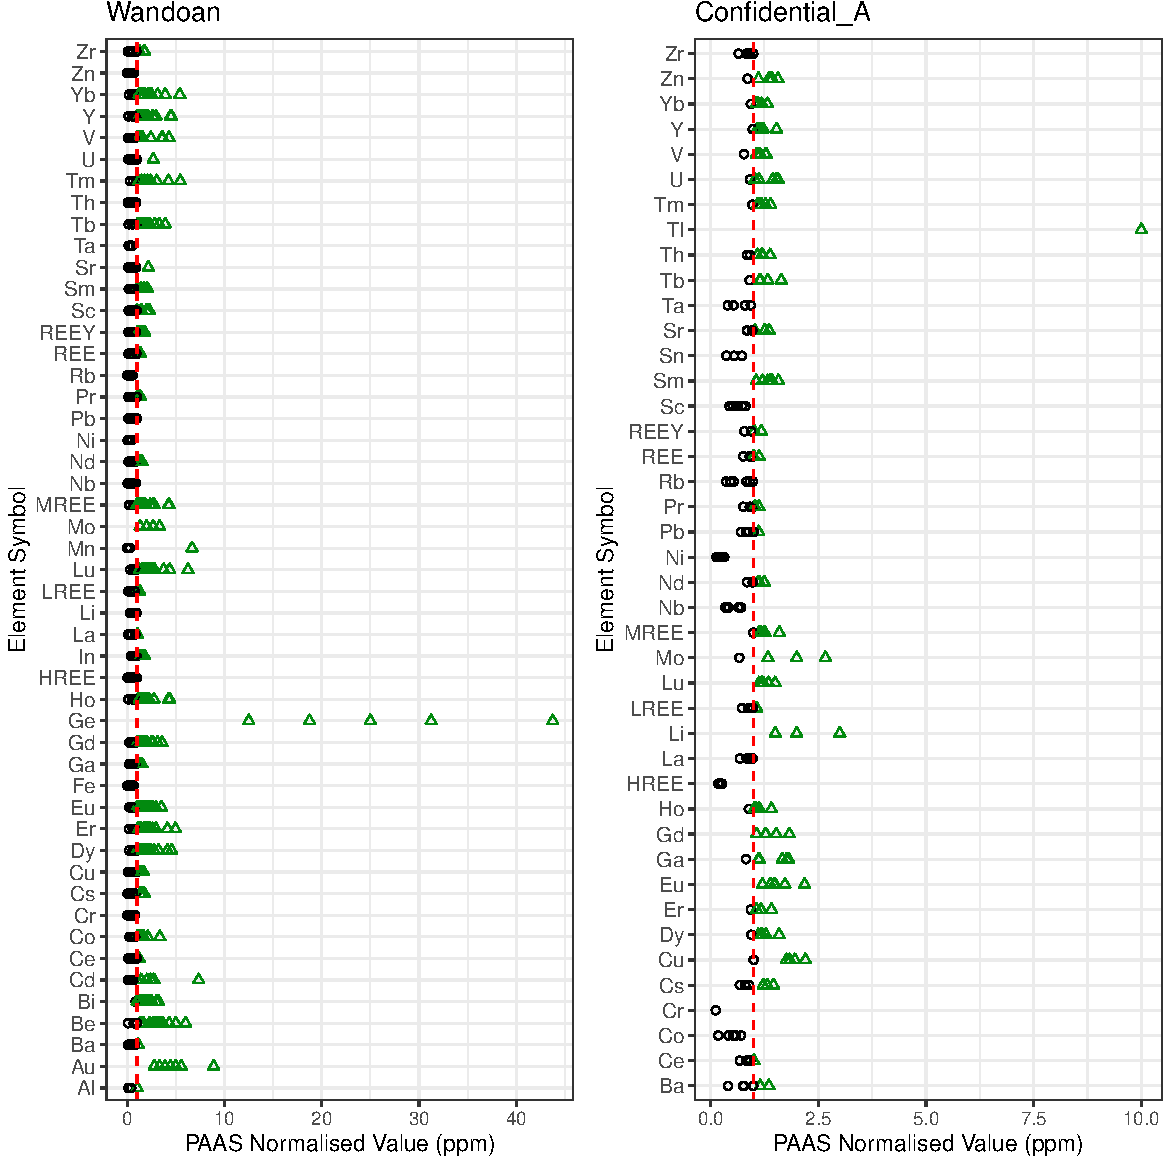
\includegraphics[width=1\linewidth,height=1\textheight]{Final_report_files/figure-latex/regionalbk6-1} \caption{Project breakdown for the distribution of element concentration with reference to PASS levels}\label{fig:regionalbk6}
\end{figure}

\newpage

\printbibliography[title=Reference]

\end{document}
